% Reconstruído de artigos/artigo_2/Artigo_2.tex


\renewcommand{\abstractname}{Resumo}
\begin{abstract}Estudamos os custos aritméticos, a seleção exata e os limites de interpolação de montagens racionais em árvores diádicas. Sob um calibre explícito, a biblioteca contém $\Theta(H^6)$ átomos; o gerador aritmético tem pior índice $\Theta(H^8)$ e a enumeração por altura realiza o mínimo exato do maior índice. Três formatos prefix-free distinguem endereços, estrutura ReLU e expansão racional. Em classes limitadas de $C^2$, a restrição de curvatura fornece um codebook com entropia de ordem $\varepsilon^{-1/2}$. Pares racionais de fronteira são estados suficientes para selecionar simultaneamente árvore e átomos, com penalidades de descrição ou orçamentos de folhas. Demonstramos as recorrências, a compatibilidade do desempate e cotas de complexidade, incluindo crescimento dos operandos. Para interpolação real em árvores estritamente diádicas, obtemos o envelope assintótico $[I(f)^2/8,\allowbreak I(f)^2/2]$. A curvatura constante realiza o intervalo completo de acumulação, e quadráticas por partes admitem uma lei periódica de fases.\end{abstract}
\renewcommand{\abstractname}{Abstract}
\begin{abstract}We study arithmetic costs, exact selection, and interpolation limits for rational assemblies on dyadic trees. Under an explicit height gauge, the library contains $\Theta(H^6)$ atoms. The arithmetic generator has worst index $\Theta(H^8)$, whereas height ordering attains the exact minimum worst index. Three prefix-free formats distinguish addresses, ReLU structure, and expanded rational coefficients. Curvature constraints yield a codebook with entropy of order $\varepsilon^{-1/2}$ on bounded $C^2$ classes. Rational boundary pairs provide sufficient states for joint tree and atom selection under description penalties or leaf budgets. We prove the recurrences, canonical tie-breaking, and complexity bounds, including operand growth. For real interpolation on strictly dyadic trees, we obtain the asymptotic envelope $[I(f)^2/8,\allowbreak I(f)^2/2]$. Constant curvature attains the full cluster interval, and piecewise quadratics admit a periodic phase law.\end{abstract}
\renewcommand{\abstractname}{Resumo}
\section{Introdução}
A aproximação por segmentos racionais envolve erro, número de folhas, altura dos coeficientes e comprimento da descrição. A seleção de uma montagem acrescenta um problema de otimização: valores em fronteiras compartilhadas acoplam decisões locais. Este artigo reúne a contagem desses recursos e as recorrências que realizam o mínimo em catálogos finitos.

A construção da biblioteca e sua semântica de endereçamento foram estabelecidas no primeiro artigo \citep{artigo_2-oliveiraI}. A codificação e a entropia se apoiam na teoria clássica de informação e aproximação \citep{artigo_1-kolmogorov1959,artigo_1-elias1975,artigo_1-cohen2001,artigo_1-cover2006}. A seleção em árvores se relaciona a partições recursivas e aproximação adaptativa \citep{artigo_2-breiman1984,artigo_2-donoho1997,artigo_2-blanchard2007,artigo_1-binev2004}. Aqui, o estado conserva os dois valores externos de cada subárvore e a admissibilidade aritmética das folhas.

O desenvolvimento liga três problemas. A contagem por altura determina o custo de endereçamento. O alfabeto racional finito permite otimizar a árvore e seus rótulos por programação dinâmica. Por fim, a restrição estritamente diádica introduz fases no erro interpolatório, mesmo antes de racionalizar os valores nodais. A referência de nós livres vem da teoria de splines \citep{artigo_1-deboor1973,artigo_1-burchard1974}; a análise diádica determina o intervalo de acumulação e sua lei de fase.

As provas de seleção exata pressupõem avaliação e comparação exatas dos custos locais. Os experimentos registrados verificam instâncias finitas dessas identidades. Os teoremas de interpolação usam valores nodais reais; sua realização racional depende também da altura. A teoria de taxas e a reversibilidade são desenvolvidas no terceiro artigo da série.

\section{Biblioteca racional e preliminares}
\label{artigo_2:sec:indexing}\label{artigo_2:sec:generator}\label{artigo_2:sec:assemblies}
Fixamos as convenções do primeiro artigo \citep{artigo_2-oliveiraI}. Para uma fração reduzida $p/q$, $q>0$, escreva $\height(p/q)=\max\{|p|,q\}$. A enumeração $Q:\Nzero\to\mathbb Q$ ordena as frações por altura, depois por denominador e numerador; $Q^*:\Nzero\to\Qstar$ omite $0$.
\begin{equation}
 Q:\Nzero\longrightarrow\mathbb Q,\qquad Q^*:\Nzero\longrightarrow\Qstar.
 \label{artigo_2:eq:q-enums}
\end{equation}
% MAPA artigo_2:2.1
\begin{lemma}[indexação elementar]\label{map:artigo_2:2.1}
\label{artigo_2:lem:cantor}\label{artigo_2:lem:integers}\label{artigo_2:lem:rational-count}\label{artigo_2:lem:rational-rank}
O pareamento $\pi(u,v)=(u+v)(u+v+1)/2+v$ é bijetivo e satisfaz $\pi(u,v)\le(u+v+1)^2$. A bijeção $Z(2j)=j$, $Z(2j+1)=-j-1$ satisfaz $Z^{-1}(m)\le2|m|+1$. Se $\mathcal Q_H=\{r:\height(r)\le H\}$, então
\[
 |\mathcal Q_H|\le3H^2,\qquad |\mathcal Q_H|\ge H^2/4\quad(H\text{ suficientemente grande}).
\]
Os postos de elementos de $\mathcal Q_H$ em $Q$ e $Q^*$ são menores que $3H^2$.
\end{lemma}
\begin{proof}
As diagonais $u+v=w$ ocupam os blocos consecutivos $[w(w+1)/2,(w+1)(w+2)/2)$. Essa decomposição fornece a inversa e a cota de $\pi$. A fórmula de $Z$ percorre separadamente inteiros não negativos e negativos. Há no máximo $(2H+1)H\le3H^2$ pares de numerador e denominador. Para a cota inferior, as frações $1\le p\le q\le H$ reduzidas são contadas por $\sum_{q\le H}\varphi(q)=3H^2/\pi^2+O(H\log H)$ \citep{artigo_1-hardy2008}. A ordem por altura limita os postos pela cardinalidade da truncagem.
\end{proof}

Para $k\in\Nzero$ e $m\in\mathbb Z$, sejam
\[
 J_{k,m}=[m2^{-k},(m+1)2^{-k}],\qquad x_{k,m}=(m+1/2)2^{-k}.
\]
% MAPA artigo_2:2.2
\begin{definition}[átomos e montagens]\label{map:artigo_2:2.2}\label{artigo_2:def:assembly}\label{artigo_2:thm:dictionary}\label{artigo_2:lem:cell-recovery}
A biblioteca $\Library$ consiste nos segmentos
\[
 \ell(x)=y_0+s(x-x_{k,m}),\qquad x\in J_{k,m},\quad y_0\in\mathbb Q,\ s\in\Qstar.
\]
Seu endereço é $\Gamma^{-1}(\ell)=\pi(\pi(k,Z^{-1}(m)),\pi(Q^{-1}(y_0),(Q^*)^{-1}(s)))$. A interface $(a,b,[c,d])$ transmite a reta $a+bx$ e sua imagem no suporte. Como $b=s\ne0$, a pré-imagem de $[c,d]$ recupera a célula. O comprimento e o extremo esquerdo recuperam $k,m$; a reta recupera $y_0,s$. Logo o endereço é único.

Uma montagem em uma raiz diádica $K$ é uma função contínua obtida por átomos nas folhas de uma árvore binária diádica cheia e finita. Denote por $\Aclass(K)$ a classe dessas funções. A convenção de posse é semiaberta à direita, exceto na folha que contém o extremo direito de $K$.
\end{definition}

% MAPA artigo_2:2.3
\begin{proposition}[densidade, interpolação e forma ReLU]\label{map:artigo_2:2.3}\label{artigo_2:prop:preliminary-facts}
As montagens são densas em $C(K)$. Se $P_Jf$ interpola $f$ nos extremos de $J$ e $f\in C^2(J)$, então
\begin{equation}
 \|f-P_Jf\|_{\infty,J}\le\frac{|J|^2}{8}\|f''\|_{\infty,J}.
 \label{artigo_2:eq:interpolation-remainder}
\end{equation}
Para uma montagem com nós $t_0<\cdots<t_N$ e inclinações $s_j$, vale, com $\rho(z)=\max\{0,z\}$,
\begin{equation}
 g(x)=g(t_0)+s_0(x-t_0)+\sum_{j=1}^{N-1}(s_j-s_{j-1})\rho(x-t_j).
 \label{artigo_2:eq:assembly-relu}
\end{equation}
\end{proposition}
\begin{proof}
A interpolação em malhas diádicas uniformes converge para toda função contínua. Em cada malha, aproximam-se seus valores nodais por racionais compartilhados, escolhendo valores adjacentes distintos. A perturbação uniforme fica limitada pelo maior erro nodal, e as inclinações resultantes são racionais não nulas. Isso prova a densidade. O resto de interpolação é $f''(\xi)(x-a)(x-b)/2$; o máximo de $|(x-a)(x-b)|$ em $[a,b]$ é $|J|^2/4$. Na fórmula ReLU, cada hinge altera a inclinação por $s_j-s_{j-1}$ e preserva a continuidade. O valor inicial e as inclinações coincidem com os da montagem em todas as folhas.
\end{proof}

\begin{proposicaoSN}\label{artigo_2:prop:bridge-part1}
Seja $K=J_{k_0,m_0}$ uma célula diádica. Então a classe $\mathcal A(K)$ da definição~\ref{map:artigo_1:4.1} (cobertura finita por células diádicas com interiores disjuntos, união contendo $K$ e valores nodais coincidentes) é igual à classe $\Aclass(K)$ da definição~\ref{map:artigo_2:2.2} (folhas de uma árvore diádica cheia de raiz $K$), como conjuntos de funções em $K$. Em ambas, cada peça é um átomo de $\Library$.
\end{proposicaoSN}
\begin{proof}
Se $g\in\Aclass(K)$, as folhas da árvore têm interiores disjuntos e união $K$, e a continuidade dá os valores nodais coincidentes; logo $g\in\mathcal A(K)$. Reciprocamente, seja $\Lambda$ uma cobertura como na definição~I.4.1 e descarte as células cuja interseção com $K$ é um ponto, que não afetam $g|_K$. Duas células diádicas ou têm interiores disjuntos ou uma contém a outra; assim, cada $J\in\Lambda$ restante satisfaz $J\subseteq K$ ou $K\subsetneq J$.

Se $K\subsetneq J$ para algum $J\in\Lambda$, o interior de $J$ contém o de $K$, de modo que $J$ é a única célula restante e $g|_K=\ell_J|_K$ com $\ell_J(x)=y_0+s(x-x_J)$. Essa restrição é afim, de inclinação $s\ne0$, e seu valor $\ell_J(x_{k_0,m_0})=y_0+s(x_{k_0,m_0}-x_J)$ no centro de $K$ é racional, pois $x_J,x_{k_0,m_0}\in\mathbb D$. Logo $g|_K$ é um átomo de $\Library$ sobre $K$, isto é, a montagem com a árvore reduzida à raiz. Se todas as células restantes estão contidas em $K$, sua união é $K$ e seus interiores são disjuntos. O fecho dessa coleção por ancestrais dentro de $K$ é uma árvore diádica finita; nenhum nó interno tem apenas um filho presente, porque o interior de cada filho está coberto por folhas. Assim, a árvore é cheia e tem as células de $\Lambda$ como folhas, o que dá $g\in\Aclass(K)$.
\end{proof}
\begin{observacaoSN}
A igualdade acima é entre as classes sem orçamento. Com orçamentos de altura e de folhas, a restrição a $K$ de um átomo de uma célula $J\supsetneq K$ pode ter altura maior: em $K=[0,1/2]$, o átomo $\ell(x)=x-1/2$ de $J_{0,0}$ tem altura $2$, mas sua restrição tem $k=1$, centro $1/4$, $y_0=-1/4$ e altura $4$. Por isso a proposição~\ref{normalizacao:prop:fixed} da Parte~II, que supõe $J_a\subseteq K$ para todos os átomos usados, é o caso em que os orçamentos coincidem. Para $K$ compacto não diádico, a definição~I.4.1 é a única disponível; todos os teoremas desta Parte e da seguinte são enunciados sobre raízes diádicas, onde as duas definições coincidem.
\end{observacaoSN}

Como referência, a interpolação linear com nós livres tem constante assintótica $I(f)^2/8$, onde $I(f)=\int_K\sqrt{|f''(x)|}\,dx$, sob as hipóteses usuais de curvatura \citep{artigo_1-deboor1973,artigo_1-burchard1974}. A restrição a árvores diádicas será examinada nas \cref{artigo_2:sec:dyadic-asymptotic,artigo_2:sec:dyadic-exact-cases}.

\section{Endereços, entropia, descrição e busca}
\label{artigo_2:sec:complexity}

\subsection{Comprimento do índice canônico}

Para um átomo com parâmetros $(k,m,y_0,s)$, defina
\begin{equation}
 H=\max\{2,\ k+1,\ |m|+1,\ \height(y_0),\ \height(s)\}.
 \label{artigo_2:eq:atom-height}
\end{equation}
Escreva $\Library_H\subset\Library$ para o conjunto dos átomos de altura no máximo $H$.

% MAPA artigo_2:3.1
\begin{theorem}[cota polinomial do endereço]\label{map:artigo_2:3.1}\label{artigo_2:thm:index-bound}
O único endereço $n$ do átomo satisfaz
\begin{equation}
 n=O(H^8),\qquad \log_2(n+1)=O(\log H).
 \label{artigo_2:eq:index-bound}
\end{equation}
As constantes são universais para a enumeração fixada.
\end{theorem}

\begin{proof}
Pelo \cref{artigo_2:lem:rational-rank}, os postos $r$ de $y_0$ e $t$ de $s$ são $O(H^2)$. Pelo \cref{artigo_2:lem:integers}, $\mu=Z^{-1}(m)=O(H)$, e $k=O(H)$. A cota do \cref{artigo_2:lem:cantor} dá
\[
 u=\pi(k,\mu)=O(H^2),\qquad v=\pi(r,t)=O(H^4),
\]
e, por uma última aplicação,
\[
 n=\pi(u,v)=O\bigl((u+v+1)^2\bigr)=O(H^8).
\]
Como $H\ge2$, tomar logaritmos fornece a segunda afirmação.
\end{proof}

\subsection{Contagem por altura e consequência minimax para o endereço}

O expoente $8$ do \cref{artigo_2:thm:index-bound} resulta do aninhamento do pareamento de Cantor. A contagem por altura determina o expoente minimax do endereçamento.

% MAPA artigo_2:3.2
\begin{lemma}[cardinalidade das cascas de altura]\label{map:artigo_2:3.2}\label{artigo_2:lem:atom-count}
Para todo $H\ge2$,
\begin{equation}
 |\Library_H|\le18H^6.
 \label{artigo_2:eq:atom-count-upper}
\end{equation}
Além disso, existem uma constante universal $c_\Library>0$ e $H_1\ge2$ tais
que, para todo $H\ge H_1$,
\begin{equation}
 |\Library_H|\ge c_\Library H^6.
 \label{artigo_2:eq:atom-count}
\end{equation}
Em particular, $|\Library_H|=\Theta(H^6)$.
\end{lemma}

\begin{proof}
Pelo \cref{artigo_2:thm:dictionary}, um átomo é determinado bijetivamente pela quádrupla $(k,m,y_0,s)\in\Nzero\times\mathbb{Z}\times\mathbb{Q}\times\Qstar$, e a altura \eqref{artigo_2:eq:atom-height} limita cada coordenada separadamente. Assim
\[
 |\Library_H|=\#\{k\le H-1\}\cdot\#\{|m|\le H-1\}\cdot|\mathcal{Q}_H|\cdot|\mathcal{Q}_H\setminus\{0\}|,
\]
com $\mathcal{Q}_H$ como no \cref{artigo_2:lem:rational-count}. O primeiro fator é $H$, o segundo é $2H-1$, e os dois últimos estão entre $c_1H^2$ e $3H^2$ para $H$ grande. Logo
\[
 |\Library_H|\le H\cdot 2H\cdot 3H^2\cdot 3H^2=18H^6,
\]
\[
 |\Library_H|\ge H\cdot H\cdot c_1H^2\cdot\bigl(c_1H^2-1\bigr)\ \ge\ \frac{c_1^2}{2}H^6
\]
para todo $H$ suficientemente grande. Tome $c_\Library=c_1^2/2$.
\end{proof}

\paragraph{Dependência do expoente no calibre.}
O expoente $6$ pertence à exaustão definida por \eqref{artigo_2:eq:atom-height}, não à
biblioteca sem calibre. De fato, se os quatro orçamentos forem desacoplados,
\[
 \Library_{K_0,M_0,Y,S}
 :=\{(k,m,y_0,s):k\le K_0,\ |m|\le M_0,
       \ \height(y_0)\le Y,\ \height(s)\le S\},
\]
então a bijeção do \cref{artigo_2:thm:dictionary} dá exatamente
\[
 |\Library_{K_0,M_0,Y,S}|
 =(K_0+1)(2M_0+1)|\mathcal Q_Y|
   (|\mathcal Q_S|-1).
\]
Assim, até constantes universais e para $Y,S$ grandes, a contagem é da ordem
de $(K_0+1)(M_0+1)Y^2S^2$. O calibre
\eqref{artigo_2:eq:atom-height} acopla $K_0=M_0=H-1$ e $Y=S=H$, produzindo $H^6$;
o acoplamento $K_0=M_0=\lfloor\log_2H\rfloor$ e $Y=S=H$, por exemplo,
produziria $H^4(\log H)^2$. Portanto mudar o orçamento de resolução, extensão
espacial ou precisão aritmética muda o expoente.

% MAPA artigo_2:3.3
\begin{proposition}[ordem exata do pior endereço aritmético]\label{map:artigo_2:3.3}
\label{artigo_2:prop:gamma-exact-order}
Se
\[
 M_\Gamma(H):=\max_{a\in\Library_H}\Gamma^{-1}(a),
\]
então
\begin{equation}
 M_\Gamma(H)=\Theta(H^8).
 \label{artigo_2:eq:gamma-exact-order}
\end{equation}
Consequentemente, o comprimento da maior palavra do gerador aritmético sobre
$\Library_H$ é $8\log_2H+O(1)$ bits.
\end{proposition}

\begin{proof}
A cota superior é o \cref{artigo_2:thm:index-bound}. Para a inferior, escreva
$N_H=|\mathcal Q_H|$. Pelo \cref{artigo_2:lem:rational-count}, $N_H\ge c_1H^2$ para
$H$ suficientemente grande. Como as enumerações de \eqref{artigo_2:eq:q-enums} listam
por altura, existem $y_H\in\mathcal Q_H$ e
$s_H\in\mathcal Q_H\setminus\{0\}$ cujos postos respectivos satisfazem
\[
 r_H=N_H-1,\qquad t_H=N_H-2,
\]
e, portanto, $r_H,t_H\ge c_2H^2$ para alguma constante universal $c_2>0$.
Considere o átomo de parâmetros $(k,m,y_0,s)=(0,0,y_H,s_H)$, que pertence a
$\Library_H$. Como
\[
 \pi(x,y)=\frac{(x+y)(x+y+1)}2+y\ge\frac{(x+y)^2}{2},
\]
temos $v_H=\pi(r_H,t_H)\ge c_3H^4$. Além disso,
$\pi(0,0)=0$, de modo que o endereço desse átomo satisfaz
\[
 n_H=\pi\bigl(\pi(0,0),v_H\bigr)=\pi(0,v_H)
 \ge\frac{v_H^2}{2}\ge c_4H^8.
\]
Logo $M_\Gamma(H)=\Omega(H^8)$, que, junto da cota superior, prova
\eqref{artigo_2:eq:gamma-exact-order}. A afirmação em bits segue tomando logaritmos.
\end{proof}

% MAPA artigo_2:3.4
\begin{theorem}[cota minimax relativa ao calibre]\label{map:artigo_2:3.4}\label{artigo_2:thm:address-lower}
Seja $A:\Library\to\Nzero$ uma aplicação injetiva qualquer. Para todo $H\ge2$,
\begin{equation}
 \max_{a\in\Library_H}A(a)\ge |\Library_H|-1.
 \label{artigo_2:eq:address-pigeonhole}
\end{equation}
Consequentemente, para todo $H\ge H_1$, existe um átomo de altura no máximo
$H$ com
\begin{equation}
 A(\text{átomo})\ \ge\ c_\Library H^6-1,
 \qquad\text{logo}\qquad
 \log_2\bigl(A(\text{átomo})+1\bigr)\ \ge\ 6\log_2H-O(1).
 \label{artigo_2:eq:address-lower}
\end{equation}
Em particular, nenhum esquema de endereçamento injetivo, canônico ou não,
pode usar $o(\log H)$ bits no pior caso sobre $\Library_H$. O expoente $6$ é
o expoente minimax para a exaustão determinada por \eqref{artigo_2:eq:atom-height}.
\end{theorem}

\begin{proof}
Por injetividade, $A(\Library_H)$ é um subconjunto de $\Nzero$ com
$|\Library_H|$ elementos distintos; seu máximo é, portanto, pelo menos
$|\Library_H|-1$, o que prova \eqref{artigo_2:eq:address-pigeonhole}. Aplique então
\eqref{artigo_2:eq:atom-count} e tome logaritmos.
\end{proof}

O \cref{artigo_2:thm:address-lower} aplica o princípio da casa dos pombos à exaustão finita. A contagem do \cref{artigo_2:lem:atom-count} fornece a ordem, e a enumeração por cascas a realiza com igualdade.

% MAPA artigo_2:3.5
\begin{remark}\label{map:artigo_2:3.5}
O argumento é puramente de contagem e não usa nenhuma propriedade de $\Gamma$. Ele vale igualmente para endereçamentos que dependam de tabelas, de estado ou de escolhas arbitrárias. Combinado com a \cref{artigo_2:prop:gamma-exact-order}, mostra que o gerador aritmético $\Gamma$ usa, no pior caso, $8\log_2H+O(1)$ bits, enquanto o limite minimax é $6\log_2H+O(1)$. Logo a razão assintótica entre os comprimentos máximos das palavras é $8/6=4/3$.
\end{remark}

A enumeração por cascas realiza o expoente $6$ para esse calibre.

% MAPA artigo_2:3.6
\begin{definition}[enumeração por altura da biblioteca]\label{map:artigo_2:3.6}\label{artigo_2:def:sharp}
Para $H\ge2$, a casca $\Library_H\setminus\Library_{H-1}$ é finita e não vazia. Ordene $\Library$ listando as cascas em ordem crescente de $H$ e, dentro de cada casca, ordenando as quádruplas $(k,m,y_0,s)$ lexicograficamente por $\bigl(k,\ Z^{-1}(m),\ \rank_Q(y_0),\ \rank_{Q^*}(s)\bigr)$, onde $\rank$ denota o posto nas enumerações \eqref{artigo_2:eq:q-enums}. A bijeção resultante é denotada $\Gamma^\sharp:\Nzero\to\Library$, e $n^\sharp$ é o endereço de um átomo nessa ordem.
\end{definition}

% MAPA artigo_2:3.7
\begin{theorem}[endereço minimax exato para a exaustão]\label{map:artigo_2:3.7}\label{artigo_2:thm:sharp-optimal}
A aplicação $\Gamma^\sharp$ é uma bijeção de $\Nzero$ sobre $\Library$, computável nos dois sentidos, e para todo $H\ge2$
\begin{equation}
 \max_{a\in\Library_H}n^\sharp(a)=|\Library_H|-1\ \le\ 18H^6-1 .
 \label{artigo_2:eq:sharp-upper}
\end{equation}
Além disso, para \emph{qualquer} endereçamento injetivo $A:\Library\to\Nzero$,
\begin{equation}
 \max_{a\in\Library_H}A(a)\ \ge\ |\Library_H|-1 .
 \label{artigo_2:eq:sharp-minimax}
\end{equation}
Logo $\Gamma^\sharp$ realiza, com igualdade e para todo $H$, o mínimo possível
do maior índice no pior caso sobre $\Library_H$; em particular esse pior
índice é $\Theta(H^6)$ e seu comprimento binário é minimax-ótimo para o
calibre \eqref{artigo_2:eq:atom-height}.
\end{theorem}

\begin{proof}
Cada casca é finita pelo \cref{artigo_2:lem:atom-count} e a ordem dentro dela é total, de modo que a concatenação está bem definida e é bijetiva; a computabilidade nos dois sentidos segue de as cascas serem finitas e explicitamente enumeráveis. Por construção, $\Gamma^\sharp$ lista primeiro, e exatamente, os elementos de $\Library_H$; portanto $\Gamma^\sharp$ restrita a $\{0,\ldots,|\Library_H|-1\}$ é uma bijeção sobre $\Library_H$, o que dá a igualdade em \eqref{artigo_2:eq:sharp-upper}, e \eqref{artigo_2:eq:atom-count-upper} dá a cota numérica. A desigualdade \eqref{artigo_2:eq:sharp-minimax} é \eqref{artigo_2:eq:address-pigeonhole}: a imagem $A(\Library_H)$ tem $|\Library_H|$ elementos distintos de $\Nzero$, logo seu máximo é ao menos $|\Library_H|-1$.
\end{proof}

% MAPA artigo_2:3.8
\begin{remark}[qual endereço usar]\label{map:artigo_2:3.8}\label{artigo_2:rem:which-address}
As duas enumerações resolvem problemas diferentes e ambas são mantidas neste trabalho.
\begin{itemize}[leftmargin=1.6em]
 \item A etapa de Cantor de $\Gamma$ tem inversa fechada: três raízes quadradas inteiras recuperam $(k,\mu,r,t)$. A recuperação de $Q(r)$ e $Q^*(t)$ utiliza os decodificadores das enumerações racionais. O pior índice tem expoente $8$.
 \item $\Gamma^\sharp$ atinge o mínimo exato de \eqref{artigo_2:eq:sharp-minimax}, logo o expoente minimax $6$ para o maior índice sob o calibre fixado, mas sua inversa requer calcular cardinalidades de cascas, isto é, somas de totientes truncadas; o custo é polinomial em $H$, não constante.
\end{itemize}
Em bits, os dois esquemas coincidem em ordem: $\log_2(n+1)=\Theta(\log H)$ em ambos, e o \cref{artigo_2:thm:address-lower} mostra que nenhum outro esquema faz melhor no pior caso sobre $\Library_H$. A diferença é uma constante multiplicativa $4/3$ no comprimento da palavra.
\end{remark}

Operacionalmente, $\Gamma$ é a semântica do átomo: seu índice é descompactado
diretamente em célula, valor ancorado e inclinação, e fornece a semântica usada na avaliação. O seletor das seções seguintes usa $\Gamma^\sharp$ no desempate declarado. Já $\Gamma^\sharp$ é um
\emph{codec} para armazenamento ou transmissão sob um limite de altura
conhecido. Converter um endereço de $\Gamma$ para $\Gamma^\sharp$ significa
decodificar primeiro o átomo e recodificar a mesma quádrupla na ordem por
cascas; a conversão inversa faz o percurso oposto. Em ambos os sentidos, a
célula e a função afim selecionada permanecem exatamente as mesmas. Portanto,
a vantagem minimax de $\Gamma^\sharp$ não altera a semântica definida por
$\Gamma$.

Sob uma raiz, um domínio e uma convenção de fronteira compartilhados, os
endereços dos átomos já recuperam suas células pela
\cref{artigo_2:lem:cell-recovery}. O conjunto das células-folha determina a árvore
diádica podada ao fechá-lo por ancestrais até a raiz; a ordem espacial é
recuperada ordenando os extremos. Assim, basta transmitir $N$, $H$ e a lista
de endereços: um esqueleto separado seria redundante.

% MAPA artigo_2:3.9
\begin{theorem}[serialização condicionada de montagens]\label{map:artigo_2:3.9}\label{artigo_2:thm:assembly-serialization}
Fixe, como informação compartilhada, o domínio $K$, a raiz diádica inicial,
a convenção de fronteira e a enumeração usada. Seja $g\in\Aclass(K)$ descrita
por uma árvore diádica com $N$ folhas, e seja $H\ge2$ a maior altura de seus
átomos. Existe um fluxo de bits autodelimitado, decodificável sem conhecer
previamente $N$ ou $H$, com comprimento
\begin{align}
 L(g\mid K)
 &\le \bigl(2\lfloor\log_2N\rfloor+1\bigr)
      +\bigl(2\lfloor\log_2H\rfloor+1\bigr)
      +N\left\lceil\log_2(18H^6)\right\rceil \notag\\
 &=N\bigl(6\log_2H+O(1)\bigr)+O(\log N+\log H)
 \label{artigo_2:eq:assembly-bitrate}
\end{align}
quando os átomos são transmitidos por $\Gamma^\sharp$. Com o gerador
aritmético $\Gamma$, o termo por folha é $8\log_2H+O(1)$ bits.
\end{theorem}

\begin{proof}
Codifique $N$ e $H$, nessa ordem, pelo código gama de Elias, com comprimentos
$2\lfloor\log_2N\rfloor+1$ e
$2\lfloor\log_2H\rfloor+1$. Conhecido $H$, cada endereço de $\Gamma^\sharp$
ocupa exatamente
$b_H=\lceil\log_2(18H^6)\rceil$ bits, pois
$n^\sharp<18H^6$ pelo \cref{artigo_2:thm:sharp-optimal}. O cabeçalho $N$ informa
quantos blocos de largura $b_H$ devem ser lidos. Os endereços recuperam os
átomos e suas células; ordenar os extremos fornece a ordem espacial, e fechar
as células por ancestrais recupera a árvore podada. O domínio compartilhado
determina apenas o recorte nas extremidades. Isso prova a primeira cota e a
decodificação sem esqueleto separado. Para $\Gamma$, use
$\max_{a\in\Library_H}\Gamma^{-1}(a)=\Theta(H^8)$ da
\cref{artigo_2:prop:gamma-exact-order}.
\end{proof}

% MAPA artigo_2:3.10
\begin{remark}\label{map:artigo_2:3.10}
Sem o domínio e a convenção de fronteira compartilhados, a expressão
``descrição completa'' seria incorreta para um intervalo $K$ com extremos
reais arbitrários: esses dados têm custo próprio e não são codificáveis, em
geral, por uma palavra finita. O \cref{artigo_2:thm:assembly-serialization} explicita
precisamente a informação lateral sob a qual a taxa de bits é afirmada.
\end{remark}

\subsection{Três formatos prefix-free e propagação de altura}
\label{artigo_2:subsec:coding-formats}

As comparações de bits usam os fluxos definidos a seguir. Códigos universais para inteiros e sua relação
com comprimentos autodelimitados são clássicos
\citep{artigo_1-elias1975,artigo_1-cover2006}. Para $n\ge1$, seja
\[
 \gamma(n)=0^{\lfloor\log_2n\rfloor}\operatorname{bin}(n)
\]
o código gama de Elias, e ponha
\[
 \zeta(z)=\begin{cases}2z,&z\ge0,\\-2z-1,&z<0.
 \end{cases}
\]
Para $r=p/q$ reduzido, $q>0$, e para o diádico escrito canonicamente como
$t=u2^{-k}$, com $u$ ímpar quando $k>0$, defina
\begin{align}
 C_{\mathbb Z}(z)&=\gamma(\zeta(z)+1),\\
 C_{\rm rat}(p/q)&=C_{\mathbb Z}(p)\,\gamma(q),
 &L_{\rm rat}(p/q)&=|C_{\rm rat}(p/q)|,\label{artigo_2:eq:rational-code}\\
 C_{\rm dyad}(u,k)&=C_{\mathbb Z}(u)\,\gamma(k+1),
 &L_{\rm dyad}(u,k)&=|C_{\rm dyad}(u,k)|.
 \label{artigo_2:eq:dyadic-code}
\end{align}
Cada componente é prefix-free e a quantidade de componentes é determinada
pelo cabeçalho do objeto; logo as concatenações abaixo são decodificáveis sem
separadores. Em particular, isso declara exatamente o que significa escrever
um diádico ``estruturalmente'' ou como racional reduzido.

% MAPA artigo_2:3.11
\begin{lemma}[cálculo elementar de alturas]\label{map:artigo_2:3.11}
\label{artigo_2:lem:height-arithmetic}
Para quaisquer $r,s\in\mathbb Q$,
\begin{equation}
 \height(r\pm s)\le2\height(r)\height(s),
 \qquad
 \height(rs)\le\height(r)\height(s).
 \label{artigo_2:eq:height-arithmetic}
\end{equation}
Em particular, se ambos têm altura no máximo $H$, as cotas respectivas são
$2H^2$ e $H^2$.
Para uma montagem de altura atômica máxima $H$, todo nó interno
$t_j=u_j2^{-k_j}$ satisfaz $|u_j|\le H$ e $k_j\le H$ em sua forma reduzida;
além disso,
\begin{align}
 \height(s_j-s_{j-1})&\le2H^2,\label{artigo_2:eq:slope-jump-height}\\
 \height(s_jt_j)&\le H2^H,\label{artigo_2:eq:slope-knot-height}\\
 \height\bigl(g(t_0)-s_0t_0\bigr)&\le2^{H+1}H^2.
 \label{artigo_2:eq:intercept-height}
\end{align}
\end{lemma}

\begin{proof}
Escreva $r=p/q$ e $s=a/b$ em forma reduzida e ponha
$R=\height(r)$, $S=\height(s)$. Antes de qualquer cancelamento,
$r\pm s=(pb\pm aq)/(qb)$ e $rs=pa/(qb)$; os numeradores têm módulos no
máximo $2RS$ e $RS$, respectivamente, e os denominadores são no máximo
$RS$. Reduzir não aumenta altura, o que prova
\eqref{artigo_2:eq:height-arithmetic}. Um nó é fronteira de uma célula
$J_{k,m}$, logo sua forma não reduzida tem expoente $k\le H-1$ e numerador
$m$ ou $m+1$, de módulo no máximo $H$; redução só diminui esses dados. As
cotas \eqref{artigo_2:eq:slope-jump-height} e \eqref{artigo_2:eq:slope-knot-height} seguem da
primeira parte e de $\height(t_j)\le2^H$. Finalmente, na primeira folha,
$g(t_0)-s_0t_0=y_0-s_0x_0$; como
$\height(x_0)\le2^H$, duas aplicações das cotas de produto e soma dão
\eqref{artigo_2:eq:intercept-height}.
\end{proof}

Fixe a ordem espacial das folhas. Os três fluxos executáveis são:
\begin{enumerate}[label=(\roman*),leftmargin=2.1em]
 \item $C_{\rm atom}(g)$: $\gamma(N)$, seguido, para cada folha, de
 $\gamma(k+1)C_{\mathbb Z}(m)C_{\rm rat}(y_0)C_{\rm rat}(s)$;
 \item $C_{\rm ReLU,str}(g)$: $\gamma(N)$, o primeiro átomo na forma ancorada
 $C_{\rm dyad}(x_0)C_{\rm rat}(y_0)C_{\rm rat}(s_0)$, e os pares
 $C_{\rm dyad}(t_j)C_{\rm rat}(s_j-s_{j-1})$;
 \item $C_{\rm ReLU,rat}(g)$: $\gamma(N)$ e a forma expandida
 $C_{\rm rat}(c)C_{\rm rat}(s_0)$, seguida dos pares
 $C_{\rm rat}(t_j)C_{\rm rat}(s_j-s_{j-1})$, onde
 $c=g(t_0)-s_0t_0$.
\end{enumerate}
Denote os comprimentos respectivos por $L_{\rm atom}$,
$L_{\rm ReLU,str}$ e $L_{\rm ReLU,rat}$. O primeiro fluxo é uma alternativa
estrutural direta à serialização por $\Gamma^\sharp$ do
\cref{artigo_2:thm:assembly-serialization}; ambos têm a mesma ordem, mas não a mesma
palavra.

% MAPA artigo_2:3.12
\begin{theorem}[comparação rigorosa dos formatos]\label{map:artigo_2:3.12}
\label{artigo_2:thm:coding-formats}
Os três fluxos acima são prefix-free e possuem decodificadores exatos. Para
toda montagem com $N$ folhas e altura atômica máxima $H\ge2$,
\begin{equation}
 L_{\rm atom}(g)=O(N\log H),\qquad
 L_{\rm ReLU,str}(g)=O(N\log H),\qquad
 L_{\rm ReLU,rat}(g)=O(NH),
 \label{artigo_2:eq:coding-format-orders}
\end{equation}
com constantes universais. A última ordem é atingida conjuntamente em $N$ e
$H$: para todo $H\ge2$ e toda potência de dois $N=2^r$ com $2\le N\le H$, seja
$K=J_{H-1-r,0}$ e considere as folhas $J_{H-1,j}$, $0\le j<N$, que são
exatamente as folhas da árvore diádica cheia de profundidade $r$ com raiz $K$.
Tome em cada folha o valor central zero e a inclinação $(-1)^j$.
Essa montagem contínua em $\Aclass(K)$ tem altura $H$, e
\begin{equation}
 L_{\rm atom}=O(N\log H),\qquad
 L_{\rm ReLU,str}=O(N\log H),\qquad
 L_{\rm ReLU,rat}=\Omega(NH).
 \label{artigo_2:eq:coding-gap-family}
\end{equation}
Assim, a equivalência funcional montagem--ReLU preserva a ordem de bits sob o
formato estrutural fixado, mas não sob a expansão racional ingênua dos
diádicos. Para $N$ qualquer com $2\le N\le H$, a mesma construção com
$N'=2^{\lfloor\log_2N\rfloor}>N/2$ folhas dá uma montagem com no máximo $N$
folhas e $L_{\rm ReLU,rat}=\Omega(N'H)=\Omega(NH)$.
\end{theorem}

\begin{proof}
O código gama é prefix-free; o mapa $\zeta$ é bijetivo entre $\mathbb Z$ e
$\Nzero$, e frações reduzidas e pares diádicos canônicos são únicos. Lendo o
cabeçalho $N$, cada decodificador sabe quantos blocos seguintes consumir. No
fluxo atômico, os blocos recuperam exatamente $(k,m,y_0,s)$ de cada folha. No
fluxo ReLU estrutural, o primeiro bloco recupera $(x_0,y_0,s_0)$ e, portanto,
$c=y_0-s_0x_0$; os demais recuperam os nós e saltos de inclinação da
\cref{artigo_2:eq:assembly-relu}; o terceiro fluxo já transmite esses parâmetros
expandidos. Logo os decodificadores são exatos.

Se $|z|\le A$, então $|C_{\mathbb Z}(z)|=O(\log(1+A))$, e se
$\height(r)\le A$, então $L_{\rm rat}(r)=O(\log(1+A))$. As coordenadas dos
átomos têm tamanho $O(H)$; os pares diádicos estruturais têm numerador e
expoente $O(H)$; e os saltos têm altura $O(H^2)$ pelo
\cref{artigo_2:lem:height-arithmetic}. Isso prova as duas primeiras cotas de
\eqref{artigo_2:eq:coding-format-orders}. Na forma ingênua, cada nó pode ter
denominador $2^H$, e o intercepto pode ter altura $2^{H+1}H^2$; o
\cref{artigo_2:lem:height-arithmetic} dá $O(H)$ bits por bloco e prova a terceira cota.

Na família final, como $N=2^r\le H$ e $H\ge2$, vale $r\le\log_2H\le H-1$, de
modo que $K=J_{H-1-r,0}$ é uma célula diádica de nível $H-1-r\ge0$. Seus
$2^r$ descendentes de nível $H-1$ são $J_{H-1,j}$, $0\le j<N$, isto é, as
folhas da árvore cheia de profundidade $r$; logo a montagem pertence a
$\Aclass(K)$ (\cref{artigo_2:def:assembly}) e seu suporte é $K=[0,2^{-(H-1-r)}]$.
As duas peças adjacentes ao nó
$t_j=j2^{-(H-1)}$ assumem ali o mesmo valor
$(-1)^{j-1}2^{-H}$, logo a montagem é contínua. Como $j<N\le H$, sua altura
atômica máxima é exatamente $H$. Há ao menos $(N-2)/2$ índices internos
ímpares $j$; para eles, $t_j$ já está reduzido e tem denominador
$2^{H-1}$. Cada bloco racional correspondente custa $\Omega(H)$ bits por
\eqref{artigo_2:eq:rational-code}, e os saltos de inclinação são não nulos. Portanto
$L_{\rm ReLU,rat}=\Omega(NH)$; os blocos atômicos e os pares diádicos
estruturais custam $O(\log H)$ cada, dando as outras duas cotas. Para $N=2$,
o intercepto $c=-2^{-H}$ fornece diretamente a mesma cota $\Omega(H)$.
Isso prova \eqref{artigo_2:eq:coding-gap-family}.
\end{proof}

O escopo do teorema é a comparação das palavras sob as convenções declaradas.
Complexidade de Kolmogorov, armazenamento de um codebook compartilhado e
custos de seleção ou decodificação pertencem a modelos adicionais.

\subsection{Erro conjunto sob orçamentos de folhas e altura}
\label{artigo_2:subsec:joint-budget}

Uma função pode admitir mais de uma representação por folhas. Para não
atribuir a ela uma altura dependente de uma escolha oculta, os dois
orçamentos serão impostos à mesma representação.

% MAPA artigo_2:3.13
\begin{definition}[erro conjunto número--altura]\label{map:artigo_2:3.13}
\label{artigo_2:def:joint-error}
Para inteiros $N,H\ge2$, seja $\Aclass_{N,H}(K)$ o conjunto das funções
$g\in\Aclass(K)$ que admitem uma representação como na
\cref{artigo_2:def:assembly} com no máximo $N$ folhas e com todos os átomos em
$\Library_H$. Defina
\begin{equation}
 E_{N,H}^{\Library}(f)_\infty
 :=\inf_{g\in\Aclass_{N,H}(K)}\|f-g\|_{\infty,K},
 \qquad \inf\varnothing:=+\infty.
 \label{artigo_2:eq:joint-error}
\end{equation}
Quando o conjunto abaixo não é vazio, ponha ainda
\begin{equation}
 H_{\varepsilon,N}^{\Library}(f)
 :=\min\{H\ge2:E_{N,H}^{\Library}(f)_\infty\le\varepsilon\}.
 \label{artigo_2:eq:height-for-accuracy}
\end{equation}
\end{definition}

Assim, $N$ mede a complexidade geométrica e $H$ mede, sob o calibre
\eqref{artigo_2:eq:atom-height}, simultaneamente resolução, posição e complexidade
aritmética. A dependência desse calibre discutida após o
\cref{artigo_2:lem:atom-count} continua valendo: $H$ não é uma invariante sem escolha
de exaustão.

% MAPA artigo_2:3.14
\begin{proposition}[monotonicidade dos dois orçamentos]\label{map:artigo_2:3.14}
\label{artigo_2:prop:joint-error-monotonicity}
Para todo $f\in C(K)$ e $N,H\ge2$,
\begin{equation}
 E_{N+1,H}^{\Library}(f)_\infty\le E_{N,H}^{\Library}(f)_\infty,
 \qquad
 E_{N,H+1}^{\Library}(f)_\infty\le E_{N,H}^{\Library}(f)_\infty.
 \label{artigo_2:eq:joint-error-monotonicity}
\end{equation}
Se
\[
 E_N^{\Library}(f)_\infty
 :=\inf\{\|f-g\|_{\infty,K}:g\in\Aclass(K)
       \text{ admite no máximo $N$ folhas}\},
\]
então $E_{N,H}^{\Library}(f)_\infty\downarrow
E_N^{\Library}(f)_\infty$ quando $H\to\infty$.
\end{proposition}

\begin{proof}
As inclusões
$\Aclass_{N,H}(K)\subseteq\Aclass_{N+1,H}(K)$ e
$\Aclass_{N,H}(K)\subseteq\Aclass_{N,H+1}(K)$ provam
\eqref{artigo_2:eq:joint-error-monotonicity}. Toda representação finita tem altura
máxima finita, logo a união de $\Aclass_{N,H}(K)$ sobre $H\ge2$ é exatamente
a classe usada para definir $E_N^{\Library}$. O ínfimo sobre essa união é o
limite da sequência decrescente de ínfimos.
\end{proof}

Fixe agora $R,M>0$ e considere
\begin{equation}
 \mathcal{F}_{R,M}=\{f\in C^2[0,1]:\|f\|_\infty\le R,\
                                  \ \|f''\|_\infty\le M\}.
 \label{artigo_2:eq:function-class}
\end{equation}

% MAPA artigo_2:3.15
\begin{lemma}[controle uniforme da primeira derivada]\label{map:artigo_2:3.15}
\label{artigo_2:lem:derivative-control}
Se $f\in\mathcal F_{R,M}$ e
\begin{equation}
 C_0:=4R+\frac M2,
 \label{artigo_2:eq:derivative-constant}
\end{equation}
então $\|f'\|_\infty\le C_0$.
\end{lemma}

\begin{proof}
Para $x\in[0,1]$, escolha $a\in\{0,1\}$ com $|a-x|\ge1/2$. Taylor com
resto de Lagrange dá
\begin{equation}
 |f'(x)|
 \le\frac{|f(a)|+|f(x)|}{|a-x|}+\frac{M}{2}|a-x|
 \le4R+\frac M2=C_0.
 \label{artigo_2:eq:derivative-control}
\end{equation}
\end{proof}

% MAPA artigo_2:3.16
\begin{theorem}[controle simultâneo de erro, folhas, altura e bits]\label{map:artigo_2:3.16}
\label{artigo_2:thm:joint-budget}
Defina
\begin{equation}
 C_H:=\max\{4(R+1),\ 2(C_0+1)\}.
 \label{artigo_2:eq:joint-height-constant}
\end{equation}
Para toda potência diádica $n=2^r\ge2$ e todo
$f\in\mathcal F_{R,M}$, existe uma montagem $g_n$ com exatamente $n$
folhas tal que
\begin{align}
 \|f-g_n\|_\infty
 &\le\frac{M+4}{8n^2},
 \label{artigo_2:eq:joint-dyadic-error}\\
 \height_{\max}(g_n)&\le C_Hn^2.
 \label{artigo_2:eq:joint-dyadic-height}
\end{align}
Nos três formatos do \cref{artigo_2:thm:coding-formats}, a mesma montagem satisfaz
\begin{equation}
 L_{\rm atom}(g_n),\ L_{\rm ReLU,str}(g_n),\
 L_{\rm ReLU,rat}(g_n)=O_{R,M}(n\log(2n)).
 \label{artigo_2:eq:joint-dyadic-bits}
\end{equation}
Consequentemente, para todo inteiro $N\ge2$,
\begin{equation}
 E_{N,\lceil C_HN^2\rceil}^{\Library}(f)_\infty
 <\frac{M+4}{2N^2}.
 \label{artigo_2:eq:joint-all-N}
\end{equation}
A construção é determinística: quando $f(t_j)$ é equidistante dos dois
pontos admissíveis da grade alternada, escolhe-se o ponto menor, ou,
equivalentemente no denominador comum de \eqref{artigo_2:eq:joint-common-denominator},
o menor numerador $b_j$.
\end{theorem}

\begin{proof}
Nos nós $t_j=j/n$, $0\le j\le n$, ponha $\Delta=n^{-2}$ e use as grades
alternadas
\begin{equation}
 G_j^{(n)}=\Delta\left(\mathbb Z+\frac{j\bmod2}{2}\right).
 \label{artigo_2:eq:joint-alternating-grid}
\end{equation}
Escolha $v_j\in G_j^{(n)}$ mais próximo de $f(t_j)$; no empate, escolha o
ponto menor. Então $|v_j-f(t_j)|\le\Delta/2$, e grades consecutivas são
disjuntas, de modo que $v_{j+1}\ne v_j$. O interpolante $g_n$ desses dados
tem, portanto, $n$ peças com inclinações racionais não nulas; cada peça é um
átomo pelo \cref{artigo_2:thm:dictionary}. A estimativa de interpolação e a
estabilidade convexa nos valores nodais dão
\[
 \|f-g_n\|_\infty
 \le\frac{M}{8n^2}+\frac{1}{2n^2}
 =\frac{M+4}{8n^2},
\]
o que prova \eqref{artigo_2:eq:joint-dyadic-error}.

Resta acompanhar a aritmética sem recorrer a uma cota genérica de soma de
racionais. Escreva, de modo comum,
\begin{equation}
 v_j=\frac{b_j}{2n^2},\qquad b_j\in\mathbb Z,
 \qquad b_j\equiv j\pmod2.
 \label{artigo_2:eq:joint-common-denominator}
\end{equation}
Como $|v_j|\le R+(2n^2)^{-1}$,
\begin{equation}
 |b_j|\le2Rn^2+1.
 \label{artigo_2:eq:joint-numerator-bound}
\end{equation}
Na folha $J_{r,j}$, o valor central e a inclinação são
\begin{equation}
 y_{0,j}=\frac{b_j+b_{j+1}}{4n^2},
 \qquad
 s_j=\frac{b_{j+1}-b_j}{2n}.
 \label{artigo_2:eq:joint-atom-parameters}
\end{equation}
O numerador de $s_j$ é ímpar, portanto a segunda fração já está reduzida e é
não nula. Pelo \cref{artigo_2:lem:derivative-control},
\begin{equation}
 |b_{j+1}-b_j|
 =2n^2|v_{j+1}-v_j|
 \le2n^2\left(\frac{C_0}{n}+\frac1{n^2}\right)
 =2C_0n+2.
 \label{artigo_2:eq:joint-slope-numerator}
\end{equation}
Reduzir $y_{0,j}$ só diminui sua altura; logo
\begin{equation}
 \height(y_{0,j})\le4(R+1)n^2,
 \qquad
 \height(s_j)\le2(C_0+1)n.
 \label{artigo_2:eq:joint-parameter-heights}
\end{equation}
Além disso, $r+1\le n$ e $|j|+1\le n$. A definição
\eqref{artigo_2:eq:atom-height} e \eqref{artigo_2:eq:joint-height-constant} provam
\eqref{artigo_2:eq:joint-dyadic-height}.

Para os bits, no formato ReLU expandido o intercepto é $c=v_0$,
$\height(c)\le2(R+1)n^2$; cada nó interno tem altura no máximo $n$; e, de
\eqref{artigo_2:eq:joint-slope-numerator},
\[
 \height(s_j-s_{j-1})\le4(C_0+1)n.
\]
Assim, tanto os parâmetros atômicos quanto os parâmetros ReLU desta
construção têm altura polinomial em $n$. Nos códigos concretos
\eqref{artigo_2:eq:rational-code}--\eqref{artigo_2:eq:dyadic-code}, cada bloco usa
$O_{R,M}(\log(2n))$ bits; há $O(n)$ blocos em qualquer dos três fluxos. Isso
prova \eqref{artigo_2:eq:joint-dyadic-bits}. Observe que a cota geral
$O(NH)$ do formato racional ingênuo não é saturada por esta família: seus
nós têm denominador apenas $n$, e não $2^H$.

Por fim, dado $N\ge2$, tome $n=2^{\lfloor\log_2N\rfloor}$. Então
$N/2<n\le N$. A montagem já construída usa no máximo $N$ folhas, tem altura
no máximo $C_Hn^2\le C_HN^2$ e erro menor que
$(M+4)/(2N^2)$, provando \eqref{artigo_2:eq:joint-all-N}.
\end{proof}

% MAPA artigo_2:3.17
\begin{corollary}[altura suficiente para precisão prescrita]\label{map:artigo_2:3.17}
\label{artigo_2:cor:height-for-epsilon}
Para $\varepsilon>0$, seja
\begin{equation}
 n_\varepsilon
 =2^{\left\lceil\log_2\max\left\{2,
        \sqrt{\frac{M+4}{8\varepsilon}}\right\}\right\rceil},
 \qquad
 H_\varepsilon=\lceil C_Hn_\varepsilon^2\rceil.
 \label{artigo_2:eq:epsilon-schedule}
\end{equation}
Então, uniformemente para $f\in\mathcal F_{R,M}$,
\begin{align}
 E_{n_\varepsilon,H_\varepsilon}^{\Library}(f)_\infty
 &\le\varepsilon,\label{artigo_2:eq:epsilon-joint-error}\\
 n_\varepsilon&=O_{R,M}(\varepsilon^{-1/2}),
 &H_\varepsilon&=O_{R,M}(\varepsilon^{-1}),
 \label{artigo_2:eq:epsilon-joint-height}\\
 L_{\rm atom},\ L_{\rm ReLU,str},\ L_{\rm ReLU,rat}
 &=O_{R,M}\!\left(\varepsilon^{-1/2}
                   \log\frac{2}{\varepsilon}\right).
 \label{artigo_2:eq:epsilon-joint-bits}
\end{align}
Em particular,
$H_{\varepsilon,n_\varepsilon}^{\Library}(f)\le H_\varepsilon$.
\end{corollary}

\begin{proof}
A escolha de $n_\varepsilon$ torna o lado direito de
\eqref{artigo_2:eq:joint-dyadic-error} no máximo $\varepsilon$. A menor potência de
dois acima de um número positivo é menor que duas vezes esse número, salvo o
piso fixo $2$; as três ordens seguem então do \cref{artigo_2:thm:joint-budget}.
\end{proof}

O expoente $H_\varepsilon=O(\varepsilon^{-1})$ é mais forte que a estimativa
preliminar $O(\varepsilon^{-3/2})$: o ganho vem do denominador diádico comum
em \eqref{artigo_2:eq:joint-common-denominator} e do controle de diferenças adjacentes
por $\|f'\|_\infty$. Trata-se de uma cota superior construtiva para a altura
mínima de \eqref{artigo_2:eq:height-for-accuracy}, não de uma cota inferior ótima.

Para tornar as quatro quantidades auditáveis, a
\cref{artigo_2:tab:joint-budget-pt} usa $f_\star(x)=4x(x-1)$, $R=1$ e $M=8$. Nesse
caso $C_0=8$, $C_H=18$, o erro exato da construção é
$49/(64N^2)$ e a altura efetiva é $4N^2$. Os três comprimentos são contados
bit a bit pelos codificadores distribuídos.

\begin{table}[t]
\centering
\small
\resizebox{\linewidth}{!}{\begin{tabular}{rrrrrrrr}
\toprule
$N$ & $e_{\rm cert}$ & $e_{\rm exato}$ & $\height_{\max}$ & $H_N$ & $L_{\rm atom}$ & $L_{\rm str}$ & $L_{\rm rat}$\\
\midrule
2 & $\frac{3}{8}$ & $\frac{49}{256}$ & 16 & 72 & 77 & 59 & 37\\
4 & $\frac{3}{32}$ & $\frac{49}{1024}$ & 64 & 288 & 195 & 115 & 89\\
8 & $\frac{3}{128}$ & $\frac{49}{4096}$ & 256 & 1152 & 513 & 235 & 211\\
16 & $\frac{3}{512}$ & $\frac{49}{16384}$ & 1024 & 4608 & 1243 & 495 & 497\\
32 & $\frac{3}{2048}$ & $\frac{49}{65536}$ & 4096 & 18\,432 & 2921 & 1067 & 1159\\
64 & $\frac{3}{8192}$ & $\frac{49}{262144}$ & 16\,384 & 73\,728 & 6731 & 2329 & 2669\\
\bottomrule
\end{tabular}
}
\caption{Construção do \cref{artigo_2:thm:joint-budget} para
$f_\star(x)=4x(x-1)$. $e_{\rm cert}$ é a cota
\eqref{artigo_2:eq:joint-dyadic-error}, $e_{\rm exato}$ é obtido em aritmética
racional nos extremos e no ponto crítico de cada folha, e $H_N=18N^2$ é a
cota provada.}
\label{artigo_2:tab:joint-budget-pt}
\end{table}

\subsection{Entropia de uma classe limitada de \texorpdfstring{$C^2$}{C2}}

Se $N_\varepsilon(\mathcal{F}_{R,M})$ é o menor número de bolas de raio $\varepsilon$ em norma uniforme que cobre a classe, escreva
\[
 \mathcal{H}_\varepsilon(\mathcal{F}_{R,M})=\log_2N_\varepsilon(\mathcal{F}_{R,M}).
\]
Essa é a entropia métrica de Kolmogorov \citep{artigo_1-kolmogorov1959,artigo_1-lorentz1996}; a ordem $\varepsilon^{-1/2}$ para classes com duas derivadas limitadas é clássica, e a demonstração abaixo é incluída apenas para tornar explícitas as constantes usadas no codebook.

% MAPA artigo_2:3.18
\begin{theorem}[entropia e codebook explícito]\label{map:artigo_2:3.18}\label{artigo_2:thm:entropy}
Existem $\varepsilon_0,c,C,C_1>0$, dependentes apenas de $R$ e $M$, tais que, para $0<\varepsilon<\varepsilon_0$,
\begin{equation}
 c\varepsilon^{-1/2}
 \le\mathcal{H}_\varepsilon(\mathcal{F}_{R,M})
 \le C\varepsilon^{-1/2}.
 \label{artigo_2:eq:entropy-order}
\end{equation}
Existe também um codebook finito $\mathcal{C}_\varepsilon\subset\Aclass([0,1])$, composto somente por montagens de átomos de $\Library$, com distorção no máximo $\varepsilon$. Quando o codebook e seu decodificador são informação compartilhada, o comprimento de seu índice global de comprimento fixo é
\begin{equation}
 L_\varepsilon^{\mathrm{global}}(\mathcal C_\varepsilon)
 :=\left\lceil\log_2|\mathcal{C}_\varepsilon|\right\rceil
 \le C_1\varepsilon^{-1/2}.
 \label{artigo_2:eq:code-length}
\end{equation}
Logo esse codebook atinge em ordem a entropia métrica da classe em cardinalidade e em bits de índice global.
\end{theorem}

\begin{proof}
\emph{Cota superior em \eqref{artigo_2:eq:entropy-order}.} Tome
\[
 N=\left\lceil\sqrt{M/\varepsilon}\right\rceil+1,\qquad h=1/N,
\]
e seja $P_Nf$ o interpolante nos nós $j/N$. A estimativa local \eqref{artigo_2:eq:interpolation-remainder}, válida para intervalos arbitrários, fornece $\|f-P_Nf\|_\infty\le Mh^2/8\le\varepsilon/8$. Quantize cada $v_j=f(j/N)$ no múltiplo mais próximo de $\Delta=\varepsilon/4$, obtendo $v'_j$ com $|v'_j-v_j|\le\varepsilon/8$. O interpolante quantizado $g$ satisfaz $\|f-g\|_\infty\le\varepsilon/4<\varepsilon$.

Resta contar os vetores quantizados que podem ocorrer. Há $O(\varepsilon^{-1})$ escolhas para $v'_0$. Dado $v'_0$, \eqref{artigo_2:eq:derivative-control} implica
\[
 |v'_1-v'_0|\le C_0h+\varepsilon/4,
\]
e portanto há $O((N\varepsilon)^{-1})=O(\varepsilon^{-1/2})$ escolhas para $v'_1$. Para $1\le j\le N-1$, a identidade integral
\[
 v_{j+1}-2v_j+v_{j-1}
 =\int_0^h\int_0^h
 f''((j-1)h+s+t)\dd s\dd t
\]
dá módulo no máximo $Mh^2\le\varepsilon$. A quantização altera a diferença segunda em no máximo $4(\varepsilon/8)=\varepsilon/2$. Dados $v'_{j-1}$ e $v'_j$, o próximo valor está, pois, em um intervalo de comprimento $3\varepsilon$, que contém no máximo uma constante universal $K$ de pontos da grade de passo $\varepsilon/4$. Consequentemente, o número total de vetores é
\[
 O(\varepsilon^{-1})\,O(\varepsilon^{-1/2})\,K^N
 =\exp\bigl(O(\varepsilon^{-1/2})\bigr),
\]
e a cota superior segue ao tomar $\log_2$.

\emph{Cota inferior em \eqref{artigo_2:eq:entropy-order}.} Fixe $\psi\in C_c^2(0,1)$ com $\|\psi\|_\infty=1$. Ponha $A=4\varepsilon$ e
\[
 w=\sqrt{\frac{A\|\psi''\|_\infty}{M}}.
\]
Para $\varepsilon$ pequeno, $A\le R$ e cabem $m=\lfloor1/w\rfloor\asymp\varepsilon^{-1/2}$ intervalos consecutivos de largura $w$ em $[0,1]$. Se $a_j=(j-1)w$, defina
\[
 \varphi_j(x)=A\psi\!\left(\frac{x-a_j}{w}\right),\qquad
 f_S=\sum_{j\in S}\varphi_j,\quad S\subset\{1,\ldots,m\}.
\]
Os suportes são disjuntos, $\|f_S\|_\infty\le A\le R$ e $\|f_S''\|_\infty\le M$. Se $S\neq T$, então $\|f_S-f_T\|_\infty=A=4\varepsilon$. Logo os $2^m$ elementos formam um empacotamento $4\varepsilon$-separado; uma bola de raio $\varepsilon$ contém no máximo um deles. Assim, $N_\varepsilon\ge2^m$ e $\mathcal{H}_\varepsilon\ge m\ge c\varepsilon^{-1/2}$.

\emph{Codebook de montagens.} Seja $N=2^k$ a menor potência de dois com $M/(8N^2)\le\varepsilon/2$. Pela minimalidade da potência de dois, $N=\Theta(\varepsilon^{-1/2})$ e $h=N^{-1}=\Theta(\varepsilon^{1/2})$. Defina
\[
 \delta=2^{-\lceil\log_2(1/\varepsilon)\rceil},
 \qquad \varepsilon/2<\delta\le\varepsilon,
\]
e, no nó $t_j=j/N$, use a grade finita alternada
\begin{equation}
 G_j=\delta\left(\mathbb{Z}+\frac{j\bmod2}{2}\right)
 \cap[-R-\delta,R+\delta].
 \label{artigo_2:eq:alternating-grid}
\end{equation}
Para cada $f$, escolha em $G_j$ um ponto $v_j$ mais próximo de $f(t_j)$, com desempate determinístico. Então $|v_j-f(t_j)|\le\delta/2$. As grades de paridades opostas são disjuntas, de modo que $v_{j+1}\neq v_j$. Como $N$ e $\delta$ são diádicos, o interpolante $g$ dos dados $(t_j,v_j)$ é uma montagem de átomos. Além disso,
\[
 \|f-g\|_\infty
 \le\|f-P_kf\|_\infty+\|P_kf-g\|_\infty
 \le\frac{M}{8N^2}+\frac\delta2\le\varepsilon.
\]
Defina $\mathcal C_\varepsilon$ como a imagem desse mapa de quantização.
É exatamente o mesmo conjunto finito de interpolantes; resta apenas contá-lo
usando a restrição de curvatura, em vez de contar todos os vetores da grade.
Há $O(\varepsilon^{-1})$ escolhas para $v_0$. Dado $v_0$, o controle
\eqref{artigo_2:eq:derivative-control} e os erros de quantização dão
\[
 |v_1-v_0|\le C_0h+\delta,
\]
de modo que há $O(h/\delta+1)=O(\varepsilon^{-1/2})$ escolhas para $v_1$.
Para $1\le j\le N-1$, a identidade de diferença segunda já usada acima e
$Mh^2\le4\varepsilon$ implicam
\[
 |v_{j+1}-2v_j+v_{j-1}|
 \le Mh^2+2\delta\le6\varepsilon.
\]
Fixados $v_{j-1}$ e $v_j$, o valor $v_{j+1}$ fica, portanto, confinado a um
intervalo de comprimento $12\varepsilon$. Os pontos de $G_{j+1}$ têm passo
$\delta>\varepsilon/2$, logo esse intervalo contém no máximo uma constante
universal $K$ de candidatos; por exemplo, $K=25$ serve. Consequentemente,
\[
 |\mathcal C_\varepsilon|
 \le C\varepsilon^{-1}\,C'\varepsilon^{-1/2}\,K^{N-1},
\]
e, como $N=O(\varepsilon^{-1/2})$,
\[
 \log_2|\mathcal C_\varepsilon|
 \le O(\log(1/\varepsilon))+N\log_2K
 =O(\varepsilon^{-1/2}).
\]
Isso prova \eqref{artigo_2:eq:code-length} sem alterar os átomos, as grades alternadas
ou a garantia de distorção.
\end{proof}

\subsection{Cinco recursos distintos: cobertura, bits, serialização, seleção e decodificação}

Para impedir que uma afirmação informacional seja interpretada como uma
afirmação algorítmica, fixemos as noções usadas daqui em diante. Seja
$(X,d)$ um espaço métrico, $\mathcal F\subset X$ totalmente limitado e
$\varepsilon>0$.

% MAPA artigo_2:3.19
\begin{definition}[recursos de um codec]\label{map:artigo_2:3.19}\label{artigo_2:def:coding-resources}
Um $\varepsilon$-codec para $\mathcal F$ é uma tripla
$(\mathcal W,\mathsf{Enc},\mathsf{Dec})$, na qual $\mathcal W$ é um conjunto
finito de palavras binárias, $\mathsf{Enc}:\mathcal F\to\mathcal W$ e
$\mathsf{Dec}:\mathcal W\to X$ satisfazem
\[
 \sup_{f\in\mathcal F}d\bigl(f,\mathsf{Dec}(\mathsf{Enc}(f))\bigr)
 \le\varepsilon.
\]
O decodificador é compartilhado e seu armazenamento não é contado no
comprimento das palavras. Distinguem-se:
\begin{align*}
 \mathcal H_\varepsilon(\mathcal F)
  &=\log_2N_\varepsilon(\mathcal F),
  &&\text{entropia métrica;}\\
 L_\varepsilon^{\mathrm{dec}}(\mathcal F)
  &=\inf_{\text{$\varepsilon$-codecs prefix-free}}
    \max_{w\in\mathcal W}|w|,
  &&\text{menor comprimento máximo decodificável;}\\
 L_\varepsilon^{\mathrm{global}}(\mathcal C_\varepsilon)
  &=\left\lceil\log_2|\mathcal C_\varepsilon|\right\rceil,
  &&\text{índice fixo em um codebook compartilhado.}
\end{align*}
Para um codebook de montagens e uma convenção de serialização fixada, ponha
\begin{align*}
 L^{\mathrm{folhas}}(g\mid K)
   &=L_{\mathrm{arv}}(g\mid K)
     +\sum_{J\in\Lambda(g)}L_{\mathrm{addr}}(g|_J),\\
 L_\varepsilon^{\mathrm{folhas}}(\mathcal C_\varepsilon\mid K)
   &=\max_{g\in\mathcal C_\varepsilon}L^{\mathrm{folhas}}(g\mid K).
\end{align*}
Por fim, depois de fixados um modelo de computação $\mathfrak M$, uma
representação de entrada para $f$ e o codec, $T_\varepsilon^{\mathrm{enc}}$
é o custo de selecionar/produzir a palavra e $T_\varepsilon^{\mathrm{dec}}$ é
o custo de reconstruí-la. Sem essas três escolhas, os dois custos temporais
não são quantidades matematicamente definidas.
\end{definition}

O símbolo ``global'' significa comprimento do \emph{índice} em uma tabela
compartilhada, não o número de bits necessário para armazenar a tabela inteira.
O símbolo ``dec'' em $L_\varepsilon^{\mathrm{dec}}$ qualifica a palavra como
decodificável; ele não representa tempo de decodificação.

% MAPA artigo_2:3.20
\begin{proposition}[limite informacional para representação decodificável]\label{map:artigo_2:3.20}
\label{artigo_2:prop:description-lower}
Todo $\varepsilon$-codec de comprimento fixo $\ell$ para $\mathcal F$ satisfaz
\begin{equation}
 \ell\ge\left\lceil\mathcal H_\varepsilon(\mathcal F)\right\rceil.
 \label{artigo_2:eq:description-lower}
\end{equation}
A mesma desigualdade vale se $\mathcal W$ é prefix-free e $\ell$ é o maior
comprimento de palavra. Em particular,
\[
 L_\varepsilon^{\mathrm{dec}}(\mathcal F)
 \ge\left\lceil\mathcal H_\varepsilon(\mathcal F)\right\rceil.
\]
Sob convenções que acrescentem ou removam apenas um cabeçalho fixo, a forma
invariante é $\ell\ge\mathcal H_\varepsilon(\mathcal F)-O(1)$.
\end{proposition}

\begin{proof}
As reconstruções $\mathsf{Dec}(\mathcal W)$ formam uma cobertura de
$\mathcal F$ por bolas de raio $\varepsilon$. Portanto,
\[
 N_\varepsilon(\mathcal F)
 \le |\mathsf{Dec}(\mathcal W)|\le|\mathcal W|.
\]
No caso de comprimento fixo, $|\mathcal W|\le2^\ell$. No caso prefix-free, a
desigualdade de Kraft e $|w|\le\ell$ dão
\[
 |\mathcal W|2^{-\ell}
 \le\sum_{w\in\mathcal W}2^{-|w|}\le1,
\]
e novamente $|\mathcal W|\le2^\ell$. Tomar logaritmos prova
\eqref{artigo_2:eq:description-lower}. Essa separação entre entropia e complexidade de
descrição é a que se usa em limites informacionais para esquemas quantizados
\citep{artigo_1-bolcskei2019}.
\end{proof}

Aplicada ao \cref{artigo_2:thm:entropy}, a proposição produz a cadeia precisa
\begin{equation}
 \mathcal H_\varepsilon(\mathcal F_{R,M})
 \le L_\varepsilon^{\mathrm{dec}}(\mathcal F_{R,M})
 \le L_\varepsilon^{\mathrm{global}}(\mathcal C_\varepsilon)
 =O(\varepsilon^{-1/2}).
 \label{artigo_2:eq:complexity-chain}
\end{equation}
Como a entropia também é $\Omega(\varepsilon^{-1/2})$, o codec é ótimo em
ordem quanto à cardinalidade, ao comprimento decodificável e aos bits do
índice global. Os custos $T_\varepsilon^{\mathrm{enc}}$ e
$T_\varepsilon^{\mathrm{dec}}$ constituem recursos computacionais separados.

Já a serialização operacional folha a folha obedece ao
\cref{artigo_2:thm:assembly-serialization}. Na construção do \cref{artigo_2:thm:entropy}, as
alturas dos parâmetros são polinomiais em $1/\varepsilon$, e por isso pode
reaparecer um custo $O(\log(1/\varepsilon))$ por folha. Esse é um custo do
formato de serialização, não da cardinalidade necessária para cobrir
$\mathcal F_{R,M}$.

\subsection{Catálogos finitos, minimizadores e truncagem}

Densidade não garante a existência de minimizadores sobre uma biblioteca
infinita. O fenômeno já ocorre para uma única avaliação.

% MAPA artigo_2:3.21
\begin{proposition}\label{map:artigo_2:3.21}\label{artigo_2:prop:no-minimizer}
Para $x=1/4$ e $y=\sqrt2$,
\[
 \inf\{|y-\ell_n(x)|:n\in\Nzero,\ x\in I_n^x\}=0,
\]
mas nenhum átomo realiza o ínfimo.
\end{proposition}

\begin{proof}
Para todo átomo, $a_n=y_{0,n}-s_nx_{0,n}\in\mathbb{Q}$ e
$b_n=s_n\in\mathbb{Q}$; como $x=1/4$ é racional,
$\ell_n(x)\in\mathbb{Q}$. Portanto, $\ell_n(x)\neq\sqrt2$.

Por outro lado, dado $\eta>0$, escolha $q\in\mathbb{Q}$ com
$|q-\sqrt2|<\eta$. Use a célula $J_{2,1}=[1/4,1/2]$, de centro $x_0=3/8$,
escolha $s=1$ e $y_0=q-s(x-x_0)=q+1/8\in\mathbb{Q}$. O
\cref{artigo_2:thm:dictionary} fornece um átomo nessa célula com
$\ell_n(1/4)=q$. Assim, os erros tendem a zero, mas nenhum é zero.
\end{proof}

A correção matemática é truncar simultaneamente geometria e aritmética. Fixe
uma raiz diádica $K=J_{k_0,m_0}$ e seja $\mathfrak T_D(K)$ o conjunto das
partições obtidas por árvores binárias diádicas completas de profundidade
relativa no máximo $D$. Uma \emph{montagem representada} é um par
$R=(\Lambda,n)$ formado por $\Lambda\in\mathfrak T_D(K)$ e um endereço
$n(J)$ para cada folha, com suporte exatamente $J$ e concordância dos valores
nas fronteiras.

% MAPA artigo_2:3.22
\begin{definition}[catálogo truncado]\label{map:artigo_2:3.22}\label{artigo_2:def:finite-catalog}
Para uma montagem representada, ponha
\[
 \height_{\max}(R)=\max_{J\in\Lambda}
 \max\{2,k(J)+1,|m(J)|+1,\height(y_{0,J}),\height(s_J)\}.
\]
Se
$H\ge H_K:=\max\{2,k_0+1,|m_0|+1\}$, defina
\begin{align}
 \mathfrak R_{D,H}^{\Library}(K)
   &=\{R=(\Lambda,n):\Lambda\in\mathfrak T_D(K),\
       \height_{\max}(R)\le H\},\label{artigo_2:eq:represented-catalog}\\
 \Sigma_{D,H}^{\Library}(K)
   &=\{\operatorname{Eval}(R):R\in
       \mathfrak R_{D,H}^{\Library}(K)\}\subset\Aclass(K).
 \label{artigo_2:eq:finite-catalog}
\end{align}
Representações distintas que avaliam na mesma função correspondem, portanto,
a um único elemento de $\Sigma_{D,H}^{\Library}(K)$.
\end{definition}

Para fixar o desempate, serialize a árvore em pré-ordem com $0$ para nó
interno e $1$ para folha e, depois, escreva os endereços
$n^\sharp(J)+1$ das folhas em ordem espacial com o código gama de Elias. O
esqueleto informa quantas palavras devem ser lidas, logo o fluxo
$\operatorname{ser}_\sharp(R)$ é autodelimitado. Ordene os fluxos por
\emph{shortlex}: primeiro pelo comprimento e depois lexicograficamente. Para
cada função, retenha o menor fluxo entre todas as suas representações no
catálogo.

% MAPA artigo_2:3.23
\begin{theorem}[finitude, existência e desempate canônico]\label{map:artigo_2:3.23}
\label{artigo_2:thm:finite-catalog-minimizer}
O catálogo $\Sigma_{D,H}^{\Library}(K)$ é finito e não vazio. Mais
precisamente, se
\[
 T_0=1,\qquad T_{d+1}=1+T_d^2,
\]
então
\begin{equation}
 1\le |\Sigma_{D,H}^{\Library}(K)|
 \le |\mathfrak R_{D,H}^{\Library}(K)|
 \le T_D|\Library_H|^{2^D}<\infty.
 \label{artigo_2:eq:finite-catalog-bound}
\end{equation}
Consequentemente, para qualquer funcional
$\mathcal J:\Sigma_{D,H}^{\Library}(K)\to\mathbb R$, existe
\begin{equation}
 g^\star\in\argmin_{g\in\Sigma_{D,H}^{\Library}(K)}\mathcal J(g).
 \label{artigo_2:eq:finite-argmin}
\end{equation}
Entre todos os minimizadores, a regra do menor fluxo shortlex seleciona uma
única função e uma única representação canônica.
\end{theorem}

\begin{proof}
A recorrência de $T_D$ conta todas as formas ordenadas de árvore: ou a raiz é
folha, ou seus dois filhos recebem independentemente uma forma de profundidade
no máximo $D-1$. Cada árvore tem no máximo $2^D$ folhas e cada folha recebe
um rótulo de $\Library_H$. Ignorar as restrições de suporte e continuidade só
aumenta a contagem, o que prova a cota superior. A árvore reduzida à raiz pode
ser rotulada, por exemplo, com $y_0=0$ e $s=1$, logo o catálogo não é vazio.
A imagem de um conjunto finito por $\operatorname{Eval}$ é finita; qualquer
função real em um conjunto finito não vazio atinge seu mínimo.

Resta o desempate. Há um número finito de representações de cada função, e a
ordem shortlex é total; portanto existe um menor fluxo. A serialização é
injetiva sobre representações, pois recupera a árvore e cada endereço de
folha. Assim, dois candidatos distintos não compartilham o mesmo fluxo, e o
menor minimizador é único.
\end{proof}

% MAPA artigo_2:3.24
\begin{proposition}[consistência sob truncagem]\label{map:artigo_2:3.24}
\label{artigo_2:prop:catalog-consistency}
Se $D\le D'$ e $H\le H'$, então
\begin{equation}
 \Sigma_{D,H}^{\Library}(K)
 \subseteq\Sigma_{D',H'}^{\Library}(K).
 \label{artigo_2:eq:catalog-nesting}
\end{equation}
Para um funcional fixado na união dos catálogos, os valores mínimos são, por
isso, não crescentes em $D$ e $H$. Se o funcional possui um minimizador global
nessa união, o minimizador global de menor fluxo shortlex e sua representação
canônica pertencem a algum catálogo finito; a partir desse par de truncagens,
o seletor canônico estabiliza.
\end{proposition}

\begin{proof}
Uma representação admissível sob $(D,H)$ continua admissível quando os dois
limites aumentam, o que prova \eqref{artigo_2:eq:catalog-nesting} e a monotonicidade dos
mínimos. A ordem shortlex bem ordena as palavras binárias finitas. Logo, entre
todas as representações de todos os minimizadores globais, existe uma menor;
ela tem profundidade e altura finitas. Qualquer catálogo que já a contenha não
pode ser superado posteriormente nem no valor do funcional nem no desempate.
\end{proof}

% MAPA artigo_2:3.25
\begin{algorithm}[enumeração exata do catálogo]\label{map:artigo_2:3.25}\label{artigo_2:alg:finite-enumeration}
Para parâmetros pequenos, gere recursivamente todas as formas de
$\mathfrak T_D(K)$; em cada folha, liste somente os átomos de $\Library_H$ com
o suporte exigido; ao unir duas subárvores, descarte pares cujos valores na
fronteira diferem. Reduza representações funcionalmente idênticas ao menor
fluxo $\operatorname{ser}_\sharp$, avalie $\mathcal J$ em aritmética racional
exata e aplique o desempate shortlex.
\end{algorithm}

Esse algoritmo realiza o
\cref{artigo_2:thm:finite-catalog-minimizer}. A cota
\eqref{artigo_2:eq:finite-catalog-bound} delimita seu uso a instâncias pequenas;
eficiência assintótica, estabilidade em relação aos dados e comportamento
perto de empates são recursos adicionais \citep{artigo_1-christof2021}.

\section{Interface da biblioteca e estados de fronteira}
\label{artigo_2:sec:interface}

\subsection{Núcleo aritmético}

Fixe
\[
 J_{k,m}=[m2^{-k},(m+1)2^{-k}],
 \qquad k\in\Nzero,\quad m\in\mathbb Z,
\]
e, para $r=p/q\in\mathbb Q$ em forma reduzida com $q>0$,
\[
 \height(r)=\max\{|p|,q\}.
\]
Pelas definições da \cref{artigo_2:sec:indexing}, a biblioteca $\Library$ está em bijeção com as
quádruplas
\[
 (k,m,y_0,s)\in\Nzero\times\mathbb Z\times\mathbb Q\times\Qstar.
\]
A quádrupla determina, em $J_{k,m}$, o átomo
\begin{equation}
 \ell(x)=y_0+s(x-x_0),
 \qquad x_0=\left(m+\frac12\right)2^{-k}.
 \label{artigo_2:eq:inherited-atom}
\end{equation}
Sua altura é
\begin{equation}
 \height_{\rm at}(k,m,y_0,s)
 =\max\{2,k+1,|m|+1,\height(y_0),\height(s)\}.
 \label{artigo_2:eq:inherited-height}
\end{equation}
Escreva $\Library_H$ para os átomos de altura no máximo $H$.

As interfaces usadas pela seleção são resumidas na
\cref{artigo_2:tab:interfaces}.
\begin{table}[t]
 \centering
 \caption{Interfaces normativas da biblioteca e da seleção.}
 \label{artigo_2:tab:interfaces}
 \small
 \begin{tabularx}{\linewidth}{@{}lX@{}}
  \toprule
  símbolo & função\\
  \midrule
  $\Gamma,\Gamma^\sharp$ & endereçamentos computáveis do mesmo átomo; o
  segundo ordena por altura e fornece o posto usado no desempate\\
  $\Library,\Library_H$ & biblioteca e sua exaustão pelo calibre
  \eqref{artigo_2:eq:inherited-height}\\
  $\Aclass(K)$ & montagens contínuas de átomos em folhas diádicas\\
  $\Representations_{D,H}^{\Library}(K)$ & representações em árvores de
  profundidade relativa no máximo $D$ e altura no máximo $H$\\
  $\Sigma_{D,H}^{\Library}(K)$ & imagens funcionais dessas representações\\
  $E_{N,H}^{\Library}$ & melhor erro com os dois orçamentos impostos à mesma
  representação\\
  \bottomrule
 \end{tabularx}
\end{table}

Fixaremos uma raiz diádica
\[
 K=J_{k_0,m_0}=[\alpha,\beta]
\]
e denotaremos por $\mathcal D_D(K)$ o conjunto de seus descendentes até
profundidade relativa $D$. Uma árvore é sempre binária, ordenada e cheia:
cada nó é folha ou possui os dois filhos diádicos. Seus conjuntos de folhas
particionam $K$.

Partições binárias recursivas são a estrutura geométrica de CART e de variantes
diádicas de árvores de decisão e aproximação
\citep{artigo_2-breiman1984,artigo_2-donoho1997,artigo_2-blanchard2007}. Aqui elas recebem, além da forma
combinatória, estados racionais de fronteira derivados da biblioteca.

\subsection{Pares admissíveis}

Se $J=J_{k,m}$, escreva $h_J=2^{-k}$. Para valores $u,v\in\mathbb Q$, a única
reta com valores $u$ e $v$ nas extremidades de $J$ é
\begin{equation}
 \ell_{J;u,v}(x)
 =u+\frac{v-u}{h_J}(x-m2^{-k}).
 \label{artigo_2:eq:endpoint-line}
\end{equation}
Seu valor central e sua inclinação são
\[
 y_0=\frac{u+v}{2},
 \qquad s=2^k(v-u).
\]

% MAPA artigo_2:4.1
\begin{definition}[pares de fronteira admissíveis]\label{map:artigo_2:4.1}
\label{artigo_2:def:admissible-pairs}
Para $H\ge2$, defina $\Pairs_H(J)$ como o conjunto dos pares
$(u,v)\in\mathbb Q^2$ que satisfazem
\begin{align}
 u&\ne v,\label{artigo_2:eq:pair-nonzero}\\
 \max\!\left\{\height\!\left(\frac{u+v}{2}\right),
 \height\!\left(2^k(v-u)\right)\right\}&\le H,\label{artigo_2:eq:pair-arithmetic}\\
 k+1&\le H,\qquad |m|+1\le H.\label{artigo_2:eq:pair-geometry}
\end{align}
\end{definition}

% MAPA artigo_2:4.2
\begin{proposition}[dicionário exato de fronteiras]\label{map:artigo_2:4.2}
\label{artigo_2:prop:endpoint-dictionary}
O mapa que associa a um átomo de $\Library_H$ com suporte $J$ seus valores
nas extremidades é uma bijeção sobre $\Pairs_H(J)$. Em particular, se
\[
 \mathcal Q_H=\{r\in\mathbb Q:\height(r)\le H\},
 \qquad q_H=|\mathcal Q_H|,
\]
então
\begin{equation}
 |\Pairs_H(J)|=
 \begin{cases}
 q_H(q_H-1),&\text{se \eqref{artigo_2:eq:pair-geometry} vale},\\
 0,&\text{caso contrário}.
 \end{cases}
 \label{artigo_2:eq:pair-count}
\end{equation}
\end{proposition}

\begin{proof}
Se um átomo tem parâmetros $(k,m,y_0,s)$, seus extremos são
\[
 u=y_0-\frac{s h_J}{2},\qquad
 v=y_0+\frac{s h_J}{2}.
\]
Como $s\ne0$, tem-se $u\ne v$. As identidades inversas
\[
 y_0=\frac{u+v}{2},\qquad s=2^k(v-u)
\]
mostram que a altura atômica não excede $H$ exatamente quando
\eqref{artigo_2:eq:pair-arithmetic}--\eqref{artigo_2:eq:pair-geometry} valem. Logo os dois
mapas são inversos.

Quando a geometria é admissível, pode-se escolher livremente
$y_0\in\mathcal Q_H$ e $s\in\mathcal Q_H\setminus\{0\}$. Há
$q_H(q_H-1)$ escolhas e a bijeção impede colisões. Quando a geometria falha,
nenhum átomo sobre $J$ pertence a $\Library_H$.
\end{proof}

\subsection{Alfabeto finito dos estados}

% MAPA artigo_2:4.3
\begin{definition}[alfabeto de fronteira]\label{map:artigo_2:4.3}
\label{artigo_2:def:value-alphabet}
Defina
\begin{equation}
 \Values_{D,H}(K)
 =\bigcup_{J\in\mathcal D_D(K)}
 \{u,v:(u,v)\in\Pairs_H(J)\}.
 \label{artigo_2:eq:value-alphabet}
\end{equation}
\end{definition}

% MAPA artigo_2:4.4
\begin{lemma}[finitude e suficiência]\label{map:artigo_2:4.4}
\label{artigo_2:lem:value-alphabet}
O conjunto $\Values_{D,H}(K)$ é finito. Todo valor assumido em uma fronteira
de folha por qualquer representação de
$\Representations_{D,H}^{\Library}(K)$ pertence a
$\Values_{D,H}(K)$. Se $S_D=2^{D+1}-1$, então
\begin{equation}
 |\Values_{D,H}(K)|
 \le \min\{2S_Dq_H(q_H-1),\,2|\Library_H|\}
 \le \min\{18S_DH^4,\,36H^6\}.
 \label{artigo_2:eq:value-alphabet-bound}
\end{equation}
\end{lemma}

\begin{proof}
Cada folha é um descendente de $K$ até profundidade $D$ e é rotulada por um
átomo de $\Library_H$. A \cref{artigo_2:prop:endpoint-dictionary} coloca seus dois
valores em \eqref{artigo_2:eq:value-alphabet}, provando a suficiência. Há $S_D$ células
na árvore completa e no máximo $q_H(q_H-1)$ pares por célula; contar os dois
extremos dá a primeira cota. Alternativamente, cada valor contado é extremo
de algum átomo de $\Library_H$, o que dá $2|\Library_H|$. As estimativas
$q_H\le3H^2$ e $|\Library_H|\le18H^6$, provadas na \cref{artigo_2:sec:complexity},
concluem.
\end{proof}

Os estados globais poderão, portanto, ser escritos como pares
$(u,v)\in\Values_{D,H}(K)^2$. Estados não realizáveis recebem custo
$+\infty$. Na implementação, apenas estados realizáveis são armazenados.

O mesmo alfabeto contém os estados internos: os valores externos de uma subárvore são extremos de suas folhas laterais, e o valor compartilhado pelos filhos é uma fronteira de folha. Logo todos os estados das \cref{artigo_2:sec:fixed-dp,artigo_2:sec:variable-dp} pertencem a $\Values_{D,H}(K)$.

\subsection{As obstruções de escala e de translação}

As condições de \eqref{artigo_2:eq:pair-geometry} limitam separadamente a escala e a posição das células admissíveis.

% MAPA artigo_2:4.5
\begin{proposition}[células vazias e refinamento uniforme máximo]\label{map:artigo_2:4.5}
\label{artigo_2:prop:translation-obstruction}
Seja $K=J_{k_0,m_0}$ com $m_0\ge0$ e seja
$J=J_{k_0+r,\,2^rm_0+j}$, $0\le j<2^r$, um descendente na profundidade
relativa $r$. Então $\Pairs_H(J)\ne\varnothing$ se e somente se
\begin{equation}
 k_0+r+1\le H
 \qquad\text{e}\qquad
 2^rm_0+j+1\le H.
 \label{artigo_2:eq:two-obstructions}
\end{equation}
Em particular, o número $N_r$ de células não vazias na profundidade $r$ é
\begin{equation}
 N_r=
 \begin{cases}
 \min\{2^r,\ \max\{0,H-2^rm_0\}\},&k_0+r+1\le H,\\
 0,&k_0+r+1>H.
 \end{cases}
 \label{artigo_2:eq:nonempty-cell-count}
\end{equation}
Além disso, \emph{todas} as $2^r$ células dessa profundidade são não vazias
se e somente se
\begin{equation}
 k_0+r+1\le H
 \qquad\text{e}\qquad
 2^r(m_0+1)\le H,
 \label{artigo_2:eq:uniform-refinement-conditions}
\end{equation}
isto é,
\begin{equation}
 r\le
 \min\!\left\{H-k_0-1,\ \log_2\frac{H}{m_0+1}\right\}.
 \label{artigo_2:eq:uniform-refinement-depth}
\end{equation}
\end{proposition}

\begin{proof}
Os índices dos descendentes de $K$ na profundidade $r$ são exatamente
$2^rm_0+j$ com $0\le j<2^r$. Como $m_0\ge0$, a condição de translação
$|m|+1\le H$ equivale a $j\le H-2^rm_0-1$; quando a condição de escala
$k_0+r+1\le H$ vale, contar os inteiros $j\in\{0,\ldots,2^r-1\}$ que
satisfazem essa desigualdade dá \eqref{artigo_2:eq:nonempty-cell-count}. Se a condição
de escala falha, nenhuma célula admite átomo, o que dá a segunda linha.
Todas as células são não vazias exatamente quando a escala é admissível e o
maior índice, $2^rm_0+2^r-1$, ainda satisfaz a condição de translação. Isso é
\eqref{artigo_2:eq:uniform-refinement-conditions}, equivalente a
\eqref{artigo_2:eq:uniform-refinement-depth}. A conclusão sobre $\Pairs_H$ segue de
\eqref{artigo_2:eq:pair-geometry} e da \cref{artigo_2:prop:endpoint-dictionary}.
\end{proof}

% MAPA artigo_2:4.6
\begin{remark}[assimetria espacial do catálogo]\label{map:artigo_2:4.6}
\label{artigo_2:rem:asymmetry}
As obstruções de escala e translação impõem limiares distintos. A obstrução de escala permite profundidade
$r\le H-k_0-1$, enquanto a de translação permite refinamento uniforme apenas
até $r\le\log_2\bigl(H/(m_0+1)\bigr)$. A profundidade disponível é o menor
desses dois limiares. Para $k_0,m_0$ fixos e $H$ suficientemente grande, o
segundo cresce apenas de modo logarítmico e acaba sendo o limitante; para
outros regimes, a escala pode ser a condição ativa. Quando a translação
limita antes da escala, ela o faz de maneira \emph{espacialmente assimétrica}:
entre as células da mesma profundidade sobrevivem as de menor índice, isto é,
as mais próximas da origem no semieixo não negativo.

Um exemplo é usado adiante. Com $K=[0,1]=J_{0,0}$ e $H=4$, a profundidade
$r=2$ é uniformemente refinável, mas em $r=3$ apenas as células de índice
$m\le3$ admitem átomos: as quatro células que cobrem $[\tfrac12,1]$ têm
$m\in\{4,5,6,7\}$ e satisfazem $\Pairs_4(J)=\varnothing$. O catálogo com
$(D,H)=(3,4)$ refina $[0,\tfrac12]$ até a profundidade $3$ e
$[\tfrac12,1]$ apenas até a profundidade $2$.

Pela \eqref{artigo_2:eq:uniform-refinement-conditions}, uma malha uniforme de passo
$2^{-r}$ em $[0,1]$ está disponível para
$H\ge\max\{2,2^r\}$. Nessa malha, a altura necessária cresce linearmente em $1/h$. A \cref{artigo_2:sec:dyadic-asymptotic} separa a constante geométrica sem
truncagem da agenda necessária para realizá-la; as
seções de classes de aproximação e agendas de altura da Parte~IV incorporam esse acoplamento
aos estratos de aproximação.
\end{remark}

\section{Funcional aditivo e representação canônica}
\label{artigo_2:sec:functional}

\subsection{Dados racionais e perda local}

Considere observações
\begin{equation}
 \mathcal Z=\{(x_i,z_i,\omega_i):1\le i\le P\},
 \qquad
 x_i\in K\cap\mathbb Q,\quad z_i\in\mathbb Q,\quad
 \omega_i\in\mathbb Q_{>0}.
 \label{artigo_2:eq:rational-data}
\end{equation}
Para que uma observação em fronteira seja contada uma única vez, defina a
parte proprietária de $J=[a,b]\subseteq K=[\alpha,\beta]$ por
\begin{equation}
 J^{\own,K}=
 \begin{cases}
 [a,b),&b<\beta,\\
 [a,b],&b=\beta.
 \end{cases}
 \label{artigo_2:eq:relative-ownership}
\end{equation}
As partes proprietárias das folhas de qualquer árvore particionam $K$.
Defina a perda racional exata
\begin{equation}
 \loss_{\mathcal Z}(J;u,v)
 =\sum_{i:\,x_i\in J^{\own,K}}
 \omega_i\bigl(z_i-\ell_{J;u,v}(x_i)\bigr)^2.
 \label{artigo_2:eq:local-loss}
\end{equation}
Pela continuidade nas fronteiras, a soma dessas perdas sobre as folhas é a
perda quadrática empírica da montagem e independe da convenção de posse.

A teoria abaixo aceita qualquer família de custos locais não negativos em um
corpo ordenado computável. A escolha \eqref{artigo_2:eq:local-loss} é mantida porque
fecha uma implementação inteiramente racional. Erros integrais ou uniformes
podem ser usados quando um oráculo local exato ou certificado estiver
disponível; a \cref{artigo_2:sec:hard-budgets} trata explicitamente o caso uniforme.

\subsection{Fluxo recursivo}

Se $a$ é um átomo, denote por $n^\sharp(a)$ seu posto em $\Gamma^\sharp$ e
por $\gamma(q)$ o código gama de Elias do inteiro positivo $q$. Defina
recursivamente um fluxo binário para representações:
\begin{equation}
 \ser_{\rm rec}(R)=
 \begin{cases}
 1\,\gamma(n^\sharp(a)+1),&R\text{ é uma folha rotulada por }a,\\
 0\,\ser_{\rm rec}(R_L)\ser_{\rm rec}(R_R),
 &R\text{ tem as subárvores ordenadas }R_L,R_R.
 \end{cases}
 \label{artigo_2:eq:recursive-stream}
\end{equation}
Esse fluxo fornece ao seletor uma representação recursiva prefix-free. A
serialização condicionada da \cref{artigo_2:sec:complexity} permanece como o formato
usado nas cotas de compressão.

% MAPA artigo_2:5.1
\begin{lemma}[decodificação e aditividade]\label{map:artigo_2:5.1}
\label{artigo_2:lem:recursive-stream}
O conjunto dos fluxos \eqref{artigo_2:eq:recursive-stream} é prefix-free e cada fluxo
recupera uma única árvore rotulada. Seu comprimento $B(R)$ satisfaz
\begin{equation}
 B(a)=1+|\gamma(n^\sharp(a)+1)|,\qquad
 B(R_L\vee R_R)=1+B(R_L)+B(R_R).
 \label{artigo_2:eq:stream-additivity}
\end{equation}
\end{lemma}

\begin{proof}
O primeiro bit distingue folha de subdivisão. No primeiro caso, o código gama
é autodelimitado e recupera o endereço do único átomo. No segundo, o
decodificador chama a si mesmo duas vezes e consome exatamente as duas
subárvores ordenadas. A indução no número de nós prova unicidade da
decodificação. Se um fluxo válido fosse prefixo próprio de outro, o
decodificador terminaria antes do fim do segundo fluxo, contradizendo o
consumo exato de uma árvore. A contagem dos bits dá
\eqref{artigo_2:eq:stream-additivity}.
\end{proof}

\subsection{Objetivo e desempate}

Fixe penalidades racionais
\[
 \lambda_{\rm bits}\ge0,\qquad \lambda_{\rm split}\ge0.
\]
Para uma representação $R$, com função avaliada $g_R$, defina
\begin{equation}
 \cost_{\mathcal Z}(R)
 =\sum_{J\in\Lambda(R)}
   \loss_{\mathcal Z}\bigl(J;g_R(\inf J),g_R(\sup J)\bigr)
 +\lambda_{\rm bits}B(R)
 +\lambda_{\rm split}\,I(R),
 \label{artigo_2:eq:additive-objective}
\end{equation}
onde $\Lambda(R)$ é o conjunto de folhas e $I(R)$ é o número de nós internos.
Em uma árvore binária cheia, $I(R)=|\Lambda(R)|-1$, mas manter a notação
separada deixa visível o custo de uma decisão de subdivisão.

Perda quadrática aditiva e penalização da complexidade sobre partições
recursivas aparecem em CART e em árvores diádicas ótimas
\citep{artigo_2-breiman1984,artigo_2-donoho1997,artigo_2-blanchard2007}. Os termos de comprimento binário,
a admissibilidade aritmética das folhas e o desempate canônico em
\eqref{artigo_2:eq:additive-objective} são específicos do problema presente.

Para um par admissível $(u,v)\in\Pairs_H(J)$, seja $a(J;u,v)$ o único átomo
da \cref{artigo_2:prop:endpoint-dictionary}. Defina o custo de folha
\begin{equation}
 \Phi_H(J;u,v)=
 \loss_{\mathcal Z}(J;u,v)
 +\lambda_{\rm bits}
  \bigl(1+|\gamma(n^\sharp(a(J;u,v))+1)|\bigr),
 \label{artigo_2:eq:leaf-cost}
\end{equation}
e ponha $\Phi_H(J;u,v)=+\infty$ quando $(u,v)\notin\Pairs_H(J)$.

Empates são resolvidos pela chave total
\begin{equation}
 \kappa(R)=
 \bigl(\cost_{\mathcal Z}(R),\,
       |\ser_{\rm rec}(R)|,\,
       \ser_{\rm rec}(R)\bigr),
 \label{artigo_2:eq:tie-key}
\end{equation}
ordenada lexicograficamente, usando a ordem lexicográfica usual no último
componente. Assim, primeiro minimiza-se o funcional; depois, o fluxo mais
curto; por fim, o menor fluxo binário.

% MAPA artigo_2:5.2
\begin{lemma}[compatibilidade do desempate com a colagem]\label{map:artigo_2:5.2}
\label{artigo_2:lem:tie-concatenation}
Considere subárvores compatíveis com os mesmos estados externos, de modo que
as substituições abaixo preservem a continuidade. Se
$\kappa(R_L)\le\kappa(R'_L)$ e $\kappa(R_R)\le\kappa(R'_R)$, então
\[
 \kappa(R_L\vee R_R)\le\kappa(R'_L\vee R'_R).
\]
Em particular, substituir um filho por outro de chave menor nunca piora a
chave de nenhuma superárvore.
\end{lemma}

\begin{proof}
Na colagem, o custo é a soma dos custos dos filhos mais a mesma constante
$\lambda_{\rm bits}+\lambda_{\rm split}$, e o comprimento é
$1+B(R_L)+B(R_R)$. Logo uma desigualdade estrita em custo, ou depois em
comprimento, é preservada. Se custo e comprimento empatam, a comparação final
é entre
$0\,\ser_{\rm rec}(R_L)\ser_{\rm rec}(R_R)$ e
$0\,\ser_{\rm rec}(R'_L)\ser_{\rm rec}(R'_R)$. Como fluxos que chegam a essa
terceira coordenada têm os mesmos comprimentos nos blocos substituídos, a
ordem lexicográfica é decidida primeiro no bloco esquerdo que difere e depois
no direito. Portanto ela também é preservada. Aplicar o argumento a um filho
de cada vez prova a afirmação.
\end{proof}

\section{Programação dinâmica em uma árvore fixa}
\label{artigo_2:sec:fixed-dp}

Seja $T$ uma árvore diádica fixa, enraizada em $K$, e de profundidade
relativa no máximo $D$. Para um nó $J$ de $T$ e
$u,v\in\Values_{D,H}(K)$, denote por
\[
 \Representations_H(T_J;u,v)
\]
o conjunto das rotulações contínuas da subárvore $T_J$ por átomos de
$\Library_H$ que assumem $u$ e $v$ nas extremidades de $J$. O conjunto pode
ser vazio.

% MAPA artigo_2:6.1
\begin{definition}[recorrência para árvore fixa]\label{map:artigo_2:6.1}
\label{artigo_2:def:fixed-recurrence}
Defina $C_T(J;u,v)$ de baixo para cima. Se $J$ é folha de $T$,
\begin{equation}
 C_T(J;u,v)=\Phi_H(J;u,v).
 \label{artigo_2:eq:fixed-leaf}
\end{equation}
Se $J$ é interno, com filhos $J_L,J_R$, defina
\begin{equation}
 C_T(J;u,v)=\lambda_{\rm bits}+\lambda_{\rm split}
 +\min_{w\in\Values_{D,H}(K)}
 \{C_T(J_L;u,w)+C_T(J_R;w,v)\}.
 \label{artigo_2:eq:fixed-split}
\end{equation}
Adota-se $\min\varnothing=+\infty$ e as regras usuais para soma com
$+\infty$.
\end{definition}

O valor intermediário $w$ aparece simultaneamente como extremo direito da
subárvore esquerda e extremo esquerdo da subárvore direita. Ele é exatamente
o acoplamento de continuidade que se perderia em um estado contendo apenas a
célula; a \cref{artigo_2:fig:boundary-state} mostra essa junção.

\begin{figure}[t]
 \centering
 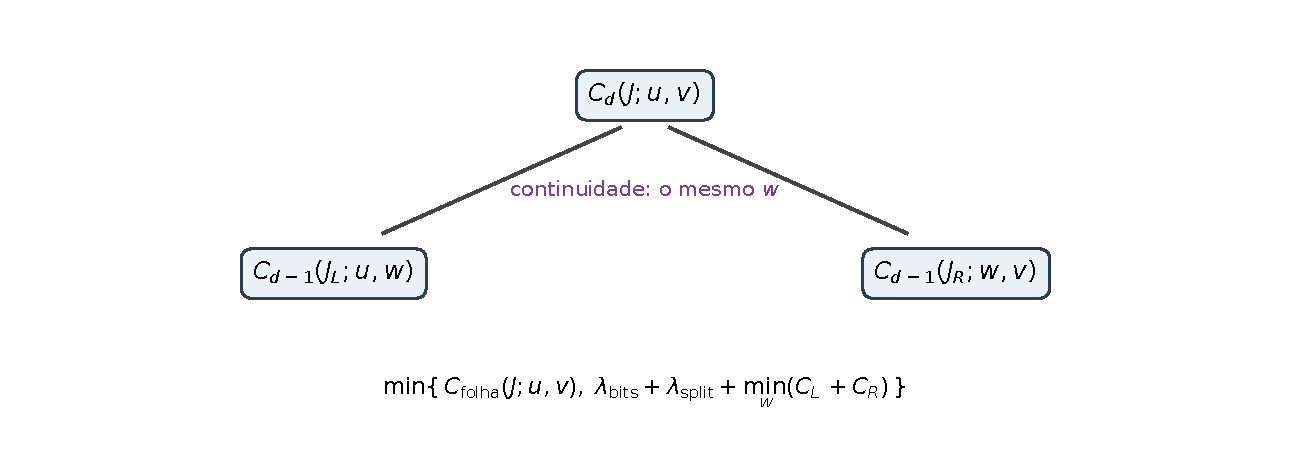
\includegraphics[width=.92\linewidth]{figuras/artigo_2/fig01_estado_fronteira.pdf}
 \caption{O estado registra os dois valores externos; o valor $w$ é
 compartilhado pelos filhos e impõe continuidade. O termo de subdivisão
 inclui o bit do nó interno e a penalidade estrutural.}
 \label{artigo_2:fig:boundary-state}
\end{figure}

% MAPA artigo_2:6.2
\begin{theorem}[correção para árvore fixa]\label{map:artigo_2:6.2}
\label{artigo_2:thm:fixed-correctness}
Para todo nó $J$ de $T$ e todo par de estados $(u,v)$,
\begin{equation}
 C_T(J;u,v)
 =\min_{R\in\Representations_H(T_J;u,v)}
 \cost_{\mathcal Z}(R),
 \label{artigo_2:eq:fixed-correctness}
\end{equation}
com valor $+\infty$ se o conjunto à direita for vazio. Se, em cada mínimo,
for armazenado também o candidato de menor chave \eqref{artigo_2:eq:tie-key}, a
retropropagação reconstrói uma única representação canônica. Em particular,
\begin{equation}
 \min_{u,v\in\Values_{D,H}(K)}C_T(K;u,v)
 =\min_{R\in\Representations_H(T)}\cost_{\mathcal Z}(R).
 \label{artigo_2:eq:fixed-global}
\end{equation}
\end{theorem}

\begin{proof}
Proceda por indução na altura da subárvore. Se $J$ é folha, a
\cref{artigo_2:prop:endpoint-dictionary} mostra que existe exatamente um rótulo com
fronteiras $(u,v)$ quando $(u,v)\in\Pairs_H(J)$, e nenhum nos demais casos.
Seu custo é precisamente \eqref{artigo_2:eq:leaf-cost}, provando
\eqref{artigo_2:eq:fixed-leaf}.

Suponha agora que $J$ tenha filhos. Toda montagem contínua em $T_J$ possui um
único valor $w$ na fronteira compartilhada. Sua restrição aos filhos pertence
a
\[
 \Representations_H(T_{J_L};u,w)
 \quad\text{e}\quad
 \Representations_H(T_{J_R};w,v).
\]
Reciprocamente, quaisquer duas representações desses conjuntos colam-se em
uma representação contínua de $T_J$. Pelo \cref{artigo_2:lem:recursive-stream}, a
colagem acrescenta um bit de nó interno; ela também acrescenta uma
subdivisão. A aditividade da perda e das duas penalidades dá
\eqref{artigo_2:eq:fixed-split}. Aplicar a hipótese de indução aos dois filhos prova
\eqref{artigo_2:eq:fixed-correctness}.

Há um número finito de estados e candidatos. A ordem de
\eqref{artigo_2:eq:tie-key} é total e, pelo \cref{artigo_2:lem:tie-concatenation}, guardar o
menor candidato em cada estado não elimina o minimizador canônico de nenhuma
superárvore. Os apontadores dos valores $w$ e das decisões recuperam esse
candidato. Minimizar também sobre os dois valores externos da raiz prova
\eqref{artigo_2:eq:fixed-global}.
\end{proof}

% MAPA artigo_2:6.3
\begin{algorithm}[rotulação exata de uma árvore fixa]\label{map:artigo_2:6.3}
\label{artigo_2:alg:fixed-tree}
Enumere $\Pairs_H(J)$ em cada folha. Percorra $T$ em pós-ordem. Em cada nó
interno, agrupe os estados do filho direito pelo valor de fronteira esquerdo
$w$ e una apenas pares com o mesmo $w$. Para cada estado externo $(u,v)$,
retenha a menor chave \eqref{artigo_2:eq:tie-key} e um apontador para os dois filhos.
Na raiz, escolha a menor entrada finita e siga os apontadores.
\end{algorithm}

O agrupamento por $w$ não altera a recorrência; ele apenas evita testar pares
de subárvores que violam continuidade de maneira evidente.

\section{Seleção simultânea da árvore e dos átomos}
\label{artigo_2:sec:variable-dp}

Para uma célula $J$ e um inteiro $d\ge0$, seja
\[
 \Representations_{d,H}(J;u,v)
\]
o conjunto das representações contínuas enraizadas em $J$, com profundidade
relativa no máximo $d$, folhas rotuladas por $\Library_H$ e valores externos
$u,v$. Diferentemente da seção anterior, a forma da árvore não é fixada.

A recorrência usa o princípio de otimalidade de \citet{artigo_2-bellman1957}. A
aproximação de curvas por segmentos via programação dinâmica já aparece em
\citet{artigo_2-bellman1961}, com antecedentes para segmentos lineares em
\citet{artigo_2-stone1961} e desenvolvimentos posteriores para aproximação poligonal
ótima em \citet{artigo_2-perezvidal1994}; aqui o estado contém os dois valores de
fronteira e a decisão de manter ou subdividir uma célula diádica.

% MAPA artigo_2:7.1
\begin{definition}[recorrência de Bellman com árvore variável]\label{map:artigo_2:7.1}
\label{artigo_2:def:variable-recurrence}
Para $d=0$, ponha
\begin{equation}
 C_0(J;u,v)=\Phi_H(J;u,v).
 \label{artigo_2:eq:variable-base}
\end{equation}
Para $d\ge1$, se $J_L,J_R$ são os filhos de $J$, defina
\begin{align}
 C_d(J;u,v)
 =\min\Bigl\{&
 \Phi_H(J;u,v),\notag\\
 &\lambda_{\rm bits}+\lambda_{\rm split}
 +\min_{w\in\Values_{D,H}(K)}
 \bigl[C_{d-1}(J_L;u,w)+C_{d-1}(J_R;w,v)\bigr]
 \Bigr\}.
 \label{artigo_2:eq:variable-recurrence}
\end{align}
\end{definition}

O primeiro ramo mantém $J$ como folha; o segundo subdivide, escolhe o valor
racional intermediário e reutiliza os ótimos dos dois filhos. A profundidade
global $D$ é usada somente para fixar um alfabeto comum suficientemente
grande; na chamada em $J$, $d$ é o número de níveis ainda disponíveis.

% MAPA artigo_2:7.2
\begin{theorem}[exatidão, existência e determinismo]\label{map:artigo_2:7.2}
\label{artigo_2:thm:variable-correctness}
Seja $J$ uma célula descendente de $K$ na profundidade relativa $r$. Para todo
$d\le D-r$ e todo $(u,v)\in\Values_{D,H}(K)^2$,
\begin{equation}
 C_d(J;u,v)
 =\min_{R\in\Representations_{d,H}(J;u,v)}
 \cost_{\mathcal Z}(R).
 \label{artigo_2:eq:variable-correctness}
\end{equation}
Consequentemente,
\begin{equation}
 C_{D,H}^{\star}(K)
 :=\min_{u,v\in\Values_{D,H}(K)}C_D(K;u,v)
 =\min_{R\in\Representations_{D,H}^{\Library}(K)}
 \cost_{\mathcal Z}(R).
 \label{artigo_2:eq:variable-global}
\end{equation}
O mínimo é finito quando
$H\ge\max\{2,k_0+1,|m_0|+1\}$. Com o desempate
\eqref{artigo_2:eq:tie-key}, o algoritmo devolve uma única representação, independentemente
da ordem em que estados, átomos ou valores intermediários sejam gerados.
\end{theorem}

\begin{proof}
A prova é por indução em $d$. Para $d=0$, apenas a árvore-folha é permitida,
e \eqref{artigo_2:eq:variable-base} coincide com seu custo ou vale $+\infty$ quando o
par é inadmissível.

Suponha o resultado para $d-1$. Toda representação de profundidade no máximo
$d$ está em exatamente um de dois casos: a raiz é folha; ou a raiz é interna
e possui duas subárvores de profundidade no máximo $d-1$. No segundo caso, a
continuidade produz um único valor compartilhado $w$. Reciprocamente, a
colagem de quaisquer duas subárvores com o mesmo $w$ é admissível. A
decomposição do custo é a mesma do \cref{artigo_2:thm:fixed-correctness}; portanto a
partição exaustiva dos candidatos nos dois casos é exatamente
\eqref{artigo_2:eq:variable-recurrence}. A hipótese de indução completa
\eqref{artigo_2:eq:variable-correctness}.

Minimizar os estados externos na raiz prova \eqref{artigo_2:eq:variable-global}. Sob a
hipótese sobre $H$, o átomo de parâmetros $(k_0,m_0,0,1)$ pertence a
$\Library_H$, logo o catálogo contém ao menos a árvore-folha e o mínimo é
finito. Todos os conjuntos examinados são finitos. A chave
\eqref{artigo_2:eq:tie-key} é total e depende somente do candidato, não da ordem de
geração, o que prova o determinismo.
\end{proof}

% MAPA artigo_2:7.3
\begin{corollary}[compatibilidade com a enumeração de formas]\label{map:artigo_2:7.3}
\label{artigo_2:cor:shape-enumeration}
Se $\Trees_D(K)$ é o conjunto finito de todas as formas de árvore de
profundidade no máximo $D$, então
\begin{equation}
 C_{D,H}^{\star}(K)
 =\min_{T\in\Trees_D(K)}
   \min_{u,v\in\Values_{D,H}(K)}C_T(K;u,v).
 \label{artigo_2:eq:shape-equivalence}
\end{equation}
O mesmo fluxo canônico vence nos dois lados.
\end{corollary}

\begin{proof}
As classes $\Representations_H(T)$, $T\in\Trees_D(K)$, particionam as
representações pela forma da árvore. Aplique os
\cref{artigo_2:thm:fixed-correctness,artigo_2:thm:variable-correctness} e o mesmo desempate
total.
\end{proof}

% MAPA artigo_2:7.4
\begin{algorithm}[seletor exato por programação dinâmica]\label{map:artigo_2:7.4}
\label{artigo_2:alg:variable-tree}
Construa as tabelas em pós-ordem na árvore diádica completa de profundidade
$D$. Inicialize cada estado com o candidato folha, quando admissível. Una as
tabelas dos filhos pelo valor intermediário $w$, acrescente o marcador e a
penalidade de subdivisão e substitua a entrada somente quando a chave completa
diminuir. A tabela da raiz e os apontadores guardados fornecem o ótimo global
e sua representação.
\end{algorithm}

\section{Orçamentos rígidos e erro uniforme}
\label{artigo_2:sec:hard-budgets}

Além do funcional penalizado, um orçamento explícito de folhas pode ser
incorporado ao estado sem alterar o princípio de otimalidade.

\subsection{Número exato de folhas}

Para $1\le n\le2^d$, defina $C_{d,n}(J;u,v)$ como o menor valor de
\eqref{artigo_2:eq:additive-objective} entre representações com exatamente $n$ folhas.
A recorrência é
\begin{align}
 C_{0,1}(J;u,v)&=\Phi_H(J;u,v),\label{artigo_2:eq:budget-base}\\
 C_{0,n}(J;u,v)&=+\infty,\qquad n>1,\notag\\
 C_{d,1}(J;u,v)&=\Phi_H(J;u,v),\qquad d\ge1,\label{artigo_2:eq:budget-one}\\
 C_{d,n}(J;u,v)&=\lambda_{\rm bits}+\lambda_{\rm split}\notag\\
 &\quad+\min_{\substack{n_L+n_R=n\\n_L,n_R\ge1}}
 \min_{w\in\Values_{D,H}(K)}
 \{C_{d-1,n_L}(J_L;u,w)+C_{d-1,n_R}(J_R;w,v)\},
 \quad n\ge2.
 \label{artigo_2:eq:budget-recurrence}
\end{align}

% MAPA artigo_2:8.1
\begin{theorem}[correção sob orçamento de folhas]\label{map:artigo_2:8.1}
\label{artigo_2:thm:leaf-budget}
As recorrências \eqref{artigo_2:eq:budget-base}--\eqref{artigo_2:eq:budget-recurrence}
calculam exatamente o menor custo entre representações de profundidade no
máximo $d$, altura no máximo $H$, fronteiras $(u,v)$ e exatamente $n$
folhas. Em particular, o ótimo com no máximo $N$ folhas é
\begin{equation}
 \min_{\substack{1\le n\le\min\{N,2^D\}\\
                  u,v\in\Values_{D,H}(K)}}
 C_{D,n}(K;u,v).
 \label{artigo_2:eq:at-most-N}
\end{equation}
\end{theorem}

\begin{proof}
A indução em $d$ é idêntica à do
\cref{artigo_2:thm:variable-correctness}, com uma coordenada adicional. Uma
representação com uma folha usa o primeiro ramo. Se possui $n\ge2$ folhas,
sua raiz é interna e as quantidades positivas de folhas dos filhos satisfazem
$n_L+n_R=n$. Reciprocamente, toda escolha listada em
\eqref{artigo_2:eq:budget-recurrence} cola duas representações com exatamente $n$
folhas. A união sobre $1\le n\le N$ prova \eqref{artigo_2:eq:at-most-N}.
\end{proof}

\subsection{Recorrência de gargalo para a norma uniforme}

Seja agora $f\in C(K)$ e suponha disponível, para cada par admissível, o erro
local exato
\begin{equation}
 e_f(J;u,v)=\|f-\ell_{J;u,v}\|_{\infty,J}.
 \label{artigo_2:eq:local-uniform-error}
\end{equation}
Quando o par é inadmissível, ponha $e_f=+\infty$. Não se supõe que esse oráculo
exista para toda apresentação de uma função contínua; para polinômios e
famílias elementares ele pode ser produzido por cálculo simbólico ou por
aritmética intervalar certificada.

Defina $B_{d,n}(J;u,v)$ substituindo soma de perdas pelo máximo entre folhas:
\begin{align}
 B_{0,1}(J;u,v)&=e_f(J;u,v),\label{artigo_2:eq:bottleneck-base}\\
 B_{0,n}(J;u,v)&=+\infty,\qquad n>1,\notag\\
 B_{d,1}(J;u,v)&=e_f(J;u,v),\label{artigo_2:eq:bottleneck-one}\\
 B_{d,n}(J;u,v)
 &=\min_{\substack{n_L+n_R=n\\n_L,n_R\ge1}}
 \min_{w\in\Values_{D,H}(K)}
 \max\{B_{d-1,n_L}(J_L;u,w),
       B_{d-1,n_R}(J_R;w,v)\}.
 \label{artigo_2:eq:bottleneck-recurrence}
\end{align}

Seja
\begin{equation}
 E_{N,H,D}^{\rm tree}(f)_\infty
 =\min\{\|f-\Eval(R)\|_{\infty,K}:
 R\in\Representations_{D,H}^{\Library}(K),\
 |\Lambda(R)|\le N\}.
 \label{artigo_2:eq:truncated-tree-error}
\end{equation}

% MAPA artigo_2:8.2
\begin{theorem}[cálculo exato do melhor erro truncado]\label{map:artigo_2:8.2}
\label{artigo_2:thm:bottleneck}
Sob o oráculo \eqref{artigo_2:eq:local-uniform-error},
\begin{equation}
 E_{N,H,D}^{\rm tree}(f)_\infty
 =\min_{\substack{1\le n\le\min\{N,2^D\}\\
                  u,v\in\Values_{D,H}(K)}}
 B_{D,n}(K;u,v).
 \label{artigo_2:eq:bottleneck-optimum}
\end{equation}
Se
\begin{equation}
 D\ge \max\{0,H-k_0-1\},
 \label{artigo_2:eq:depth-inactive}
\end{equation}
a restrição de profundidade já é inativa: nenhum átomo de $\Library_H$
apoiado em descendente de $K$ pode ocorrer abaixo desse nível.
\end{theorem}

\begin{proof}
Em uma montagem contínua, o erro uniforme global é o máximo dos erros nas
folhas. A mesma partição em raiz-folha ou raiz-interna usada no
\cref{artigo_2:thm:leaf-budget} produz
\eqref{artigo_2:eq:bottleneck-recurrence}, agora com o operador máximo na colagem.
A indução em $d$ prova que $B_{d,n}$ é o melhor gargalo com o estado e a
quantidade de folhas fixados. Minimizar essas coordenadas dá
\eqref{artigo_2:eq:bottleneck-optimum}.

Uma folha na profundidade relativa $r$ tem escala $k_0+r$. Pela altura
\eqref{artigo_2:eq:inherited-height}, sua admissibilidade exige
$k_0+r+1\le H$. Portanto $r\le H-k_0-1$, o que prova a última afirmação.
\end{proof}

% MAPA artigo_2:8.3
\begin{remark}[interação entre profundidade e translação]\label{map:artigo_2:8.3}
\label{artigo_2:rem:depth-vs-translation}
A condição \eqref{artigo_2:eq:depth-inactive} satura o ganho obtido pelo aumento de $D$
além de $H-k_0-1$. A admissibilidade de cada célula também depende de sua
posição.
Para $m_0\ge0$, a \cref{artigo_2:prop:translation-obstruction} mostra que o refinamento
uniforme completo exige também
$r\le\log_2\bigl(H/(m_0+1)\bigr)$. Quando esse segundo limiar é o menor, o
catálogo se torna espacialmente assimétrico antes de a escala se esgotar. Ao ler
\eqref{artigo_2:eq:bottleneck-optimum} para um dado $(N,H,D)$, portanto, o orçamento de
folhas $N$ compete com uma família de árvores que já está truncada pela
translação, não apenas pela profundidade.
\end{remark}

% MAPA artigo_2:8.4
\begin{corollary}[convergência para funções contínuas]\label{map:artigo_2:8.4}
\label{artigo_2:cor:uniform-convergence}
Para todo $f\in C(K)$,
\begin{equation}
 \inf_{N,H,D}E_{N,H,D}^{\rm tree}(f)_\infty=0.
 \label{artigo_2:eq:uniform-convergence}
\end{equation}
Mais precisamente, ao longo de qualquer sequência de triplas $(N,H,D)$ que
seja componente a componente não decrescente e cofinal, os erros convergem a
zero.
\end{corollary}

\begin{proof}
Os catálogos são aninhados em cada orçamento, logo os erros não crescem. O
teorema de densidade da \cref{artigo_2:sec:assemblies} afirma que, dado $\varepsilon>0$,
existe uma montagem contínua finita de átomos com erro menor que
$\varepsilon$. Essa representação possui números finitos de folhas,
profundidade e altura; portanto pertence a algum catálogo da união. Assim, o
ínfimo em \eqref{artigo_2:eq:uniform-convergence} é zero, e a monotonicidade prova a
convergência cofinal.
\end{proof}

\section{Complexidade, truncagem e estabilidade}
\label{artigo_2:sec:complexity-dp}

\subsection{Contagem de operações}

Escreva
\[
 M=|\Values_{D,H}(K)|,\qquad S_D=2^{D+1}-1.
\]
As cotas abaixo usam o modelo de custo unitário para operações e comparações
no corpo ordenado dos custos. O tamanho dos operandos racionais será discutido
separadamente. O custo do terceiro componente da chave \eqref{artigo_2:eq:tie-key}, o
\emph{fluxo binário completo}, é contado em bits. Comparar duas
chaves que empatam nas duas primeiras componentes custa
$O(L)$, onde
\begin{equation}
 L=\max_R|\ser_{\rm rec}(R)|
 \le S_D\bigl(2\lfloor\log_2|\Library_H|\rfloor+2\bigr)
 \label{artigo_2:eq:stream-length}
\end{equation}
é o comprimento máximo de fluxo no catálogo. Todas as cotas desta seção contam
comparações de chave e construção/concatenação de fluxos como unitárias;
multiplicá-las por $L$ dá uma cota superior correspondente no modelo em que
comparar ou copiar um bit tem custo unitário.
Pela mesma razão, as cotas de memória contam \emph{entradas} da tabela, e cada
entrada que armazena um fluxo ocupa até $L$ bits. Uma implementação que
guarde apenas ponteiros de reconstrução e recomponha o fluxo sob demanda
troca esse fator de memória por trabalho adicional na comparação.

% MAPA artigo_2:9.1
\begin{theorem}[complexidade em número de estados]\label{map:artigo_2:9.1}
\label{artigo_2:thm:state-complexity}
Suponha os custos de folha pré-computados. Uma implementação densa do
\cref{artigo_2:alg:variable-tree} usa
\begin{equation}
 O(S_DM^3)
 \label{artigo_2:eq:dense-time}
\end{equation}
operações e
\begin{equation}
 O(S_DM^2)
 \label{artigo_2:eq:dense-memory}
\end{equation}
entradas de memória quando preserva todos os apontadores de reconstrução.
A versão com orçamento de até $N$ folhas usa
\begin{equation}
 O(S_DN^2M^3)
 \label{artigo_2:eq:budget-time}
\end{equation}
operações e $O(S_DNM^2)$ entradas. Se cada custo local
\eqref{artigo_2:eq:local-loss} for calculado diretamente sobre $P$ observações, a
inicialização densa acrescenta $O(S_DPM^2)$ operações.
\end{theorem}

\begin{proof}
Cada nó tem no máximo $M^2$ estados externos $(u,v)$. Em um nó interno, a
recorrência testa no máximo $M$ valores intermediários $w$ por estado, logo
$O(M^3)$ operações. Há no máximo $S_D$ nós. Armazenar um custo e um apontador
por estado dá \eqref{artigo_2:eq:dense-memory}.

Com o número de folhas no estado, há $N$ camadas de custo. Somando, para todos
$n\le N$, as decomposições positivas $n_L+n_R=n$, obtêm-se $O(N^2)$ pares de
orçamentos por tripla $(u,w,v)$. Isso prova \eqref{artigo_2:eq:budget-time} e a cota de
memória. A última afirmação vem de somar até $P$ termos em cada custo local.
\end{proof}

% MAPA artigo_2:9.2
\begin{remark}[tabelas esparsas]\label{map:artigo_2:9.2}
\label{artigo_2:rem:sparse}
As cotas são deliberadamente densas. O algoritmo distribuído armazena apenas
pares realizáveis e agrupa o filho direito por $w$. Seu trabalho em um nó é
proporcional ao tamanho da junção
\[
 \#\{((u,w),(w,v)):\text{os dois estados estão presentes}\},
\]
que pode ser muito menor que $M^3$. Essa melhora depende da instância e não
altera a cota de pior caso.

Na instância principal da \cref{artigo_2:sec:numerical}, com
$(D,H)=(3,4)$, o alfabeto efetivo tem $M=475$ elementos, contra
$2S_Dq_H(q_H-1)=15\,180$ pela primeira cota de
\eqref{artigo_2:eq:value-alphabet-bound} e $36H^6=147\,456$ pela segunda; e a tabela da
raiz contém $3383$ estados realizáveis, contra $M^2=225\,625$ posições
densas, isto é, uma ocupação de $1{,}5\%$. Nas instâncias examinadas, a
estrutura esparsa reduz substancialmente o trabalho em relação à cota densa de
pior caso.
\end{remark}

\subsection{Modelo de custo e complexidade de bits}

Pelo \cref{artigo_2:lem:value-alphabet},
\[
 M\le36H^6,
\]
e portanto \eqref{artigo_2:eq:dense-time} fornece, de modo bruto,
\begin{equation}
 O(S_DH^{18})
 \label{artigo_2:eq:height-worst}
\end{equation}
operações de custo unitário. A expressão é polinomial no valor numérico de
$H$, cujo comprimento binário é $O(\log H)$, e
$S_D=2^{D+1}-1$. Trata-se, portanto, de uma cota pseudo-polinomial nos
orçamentos codificados em binário.

Para fechar também esse segundo nível, defina, para $r=p/q$ reduzido, $q>0$,
\begin{equation}
 \operatorname{bl}(r)
 :=1+\left\lceil\log_2(|p|+1)\right\rceil
    +\left\lceil\log_2(q+1)\right\rceil .
 \label{artigo_2:eq:rational-bit-length}
\end{equation}
Seja $B_{\mathcal Z}$ o maior comprimento \eqref{artigo_2:eq:rational-bit-length}
entre abscissas, respostas, pesos e penalidades racionais da instância. Denote
por $\mathsf M_{\mathbb Z}(b)$ uma cota para multiplicar inteiros de $b$ bits,
e recorde o limite $L$ de \eqref{artigo_2:eq:stream-length}.

% MAPA artigo_2:9.3
\begin{theorem}[cota grosseira de complexidade de bits]\label{map:artigo_2:9.3}
\label{artigo_2:thm:bit-complexity}
Todos os custos racionais que aparecem na recorrência possuem numeradores e
denominadores de comprimento no máximo
\begin{equation}
 B_{\rm cost}
 =O\!\left(
 P\bigl(B_{\mathcal Z}+D+|k_0|+\log(2H)\bigr)
 +B_{\mathcal Z}+D+\log(2L)
 \right).
 \label{artigo_2:eq:cost-bit-growth}
\end{equation}
Consequentemente, a versão densa sem orçamento de folhas pode ser executada em
\begin{equation}
 O\!\left(
 (S_DM^3+S_DPM^2)
 \bigl[\mathsf M_{\mathbb Z}(B_{\rm cost})
       \log(2B_{\rm cost})+L\bigr]
 \right)
 \label{artigo_2:eq:dense-bit-time}
\end{equation}
operações de bit e
\begin{equation}
 O\!\left(S_DM^2(B_{\rm cost}+L)\right)
 \label{artigo_2:eq:dense-bit-memory}
\end{equation}
bits de memória quando todos os estados e fluxos são armazenados. Na versão
com até $N$ folhas, substituem-se $S_DM^3$ e $S_DM^2$ por
$S_DN^2M^3$ e $S_DNM^2$, respectivamente. Com multiplicação escolar,
$\mathsf M_{\mathbb Z}(b)=O(b^2)$.
\end{theorem}

\begin{proof}
Um átomo admissível tem $\operatorname{bl}(y_0),
\operatorname{bl}(s)=O(\log(2H))$. Em uma célula descendente de profundidade
no máximo $D$, escrever o centro ou um extremo como racional expande o fator
diádico em no máximo $D+|k_0|+O(1)$ bits. Portanto a avaliação afim em uma
abscissa da amostra tem comprimento
\[
 O(B_{\mathcal Z}+D+|k_0|+\log(2H)).
\]
Subtrair a resposta, elevar ao quadrado e multiplicar pelo peso apenas altera
a constante dessa cota. Na soma ingênua de $P$ frações, pode-se tomar como
denominador o produto dos denominadores; logo numerador e denominador têm
comprimento no máximo $P$ vezes o maior comprimento de uma parcela. Os termos
de penalização acrescentam $O(B_{\mathcal Z}+D+\log(2L))$ bits. Isso prova
\eqref{artigo_2:eq:cost-bit-growth}; cancelamentos por máximo divisor comum só podem
reduzir os operandos.

Uma soma, comparação ou redução de frações com operandos de comprimento
$B_{\rm cost}$ custa
$O(\mathsf M_{\mathbb Z}(B_{\rm cost})\log(2B_{\rm cost}))$ operações de bit
por algoritmos inteiros usuais. Quando custos e número de folhas empatam, a
comparação shortlex lê no máximo $L$ bits. Multiplicar esse custo pelo número
de transições e inicializações do \cref{artigo_2:thm:state-complexity} dá
\eqref{artigo_2:eq:dense-bit-time}. Cada estado guarda um custo, um fluxo ou apontador
de reconstrução e índices de $O(\log(S_DM))$ bits, absorvidos pela cota exibida;
isso prova \eqref{artigo_2:eq:dense-bit-memory}. O argumento com a coordenada de
orçamento é idêntico.
\end{proof}

A cota é propositalmente conservadora: ela não explora cancelamentos nem
denominadores compartilhados. Ainda assim, fecha o modelo de Turing e torna
explícito o ponto essencial. Como $M\le36H^6$ e $S_D=2^{D+1}-1$, a
dependência continua pseudo-polinomial nos valores numéricos de $H$ e $2^D$,
mesmo após contabilizar o crescimento dos racionais.

\subsection{Valores sob truncagem}

Seja
\[
 \Representations_{\infty}^{\Library}(K)
 =\bigcup_{D,H}\Representations_{D,H}^{\Library}(K)
\]
o conjunto de todas as representações finitas enraizadas em $K$.

% MAPA artigo_2:9.4
\begin{proposition}[convergência dos mínimos penalizados]\label{map:artigo_2:9.4}
\label{artigo_2:prop:truncation-convergence}
Os valores $C_{D,H}^{\star}(K)$ de \eqref{artigo_2:eq:variable-global} são não
crescentes separadamente em $D$ e $H$, e
\begin{equation}
 \inf_{D,H}C_{D,H}^{\star}(K)
 =\inf_{R\in\Representations_{\infty}^{\Library}(K)}
   \cost_{\mathcal Z}(R).
 \label{artigo_2:eq:penalized-limit}
\end{equation}
Ao longo de qualquer sequência componente a componente não decrescente e
cofinal em $(D,H)$, os valores convergem ao lado direito.

Se o ínfimo em \eqref{artigo_2:eq:penalized-limit} é atingido, o minimizador global de
menor chave \eqref{artigo_2:eq:tie-key} pertence a algum catálogo finito; a partir de
uma truncagem que o contenha, o seletor canônico estabiliza.
\end{proposition}

\begin{proof}
Aumentar $D$ ou $H$ preserva toda representação já admissível, logo os
mínimos não crescem. A união dos domínios dos mínimos é exatamente
$\Representations_{\infty}^{\Library}(K)$, o que prova
\eqref{artigo_2:eq:penalized-limit}. Uma sequência cofinal eventualmente contém cada
representação finita; a monotonicidade conclui a convergência.

Se há minimizadores globais, seus comprimentos de fluxo formam um subconjunto
não vazio de $\Nzero$ e possuem mínimo. Entre as finitíssimas palavras desse
comprimento existe uma menor lexicograficamente. A representação
correspondente tem profundidade e altura finitas. Depois que ela entra no
catálogo, nenhum candidato posterior pode melhorar o custo ou a chave.
\end{proof}

\subsection{Um limite de estabilidade}

% MAPA artigo_2:9.5
\begin{proposition}[um seletor exato pode ser descontínuo]\label{map:artigo_2:9.5}
\label{artigo_2:prop:instability}
Considere, em $K=[0,1]$, o subcatálogo formado pelos dois átomos
\[
 g_+(x)=x,\qquad g_-(x)=-x,
\]
ambos de altura $2$. Para uma única observação $(x,z)=(1,z)$, custo igual à
perda quadrática e qualquer desempate determinístico, o mapa que envia $z$ ao
átomo selecionado é descontínuo em $z=0$ na norma uniforme.
\end{proposition}

\begin{proof}
Os custos são
\[
 \cost_z(g_+)=(z-1)^2,\qquad
 \cost_z(g_-)=(z+1)^2.
\]
Logo $g_+$ é o único minimizador para $z>0$, $g_-$ é o único minimizador para
$z<0$ e há empate em $z=0$. Qualquer regra escolhe um deles no empate, mas a
sequência que se aproxima por dados do lado oposto seleciona sempre o outro.
Como
\[
 \|g_+-g_-\|_{\infty,[0,1]}=2,
\]
não há continuidade.
\end{proof}

O exemplo separa exatidão de continuidade do seletor. Hipóteses de margem
entre custos produzem regiões de seleção localmente constante; nos empates,
uma saída a valores conjuntos preserva semicontinuidade. Essa distinção entre
existência, estabilidade e não unicidade também aparece na análise de problemas
de treinamento por perda quadrática em esquemas não lineares
\citep{artigo_1-christof2021}.

\section{Validação computacional exata}
\label{artigo_2:sec:numerical}

\subsection{Implementação}

O script
\path{verificacao/seletor_dinamico_exato.py}
implementa os \cref{artigo_2:alg:fixed-tree,artigo_2:alg:variable-tree}. O domínio numérico é
\texttt{Fraction}. As tabelas são dicionários esparsos indexados
por pares de \texttt{Fraction}; a junção dos filhos usa igualdade racional
exata no valor $w$. Perdas, penalidades, comparações de objetivo, alturas,
endereços $\Gamma^\sharp$ e desempates não usam ponto flutuante.
\texttt{NumPy} e \texttt{Matplotlib} aparecem somente depois da seleção, para
desenhar as figuras.

Cada execução verifica:
\begin{enumerate}[label=(\alph*),leftmargin=2em]
 \item a continuidade de todas as fronteiras da montagem vencedora;
 \item a altura de cada folha;
 \item a igualdade entre o ótimo da recorrência variável e o mínimo obtido ao
 enumerar separadamente todas as formas e resolver cada árvore fixa;
 \item a coincidência com uma enumeração direta de representações na
 instância mínima descrita abaixo;
 \item que uma derivação separada de $\mathcal Q_H$, dos pares de extremos
 e das perdas locais coincide com as rotinas usadas pela PD;
 \item as recorrências com número exato de folhas e de gargalo contra
 enumeração sem poda;
 \item a robustez da comparação num orçamento sem células eliminadas;
 \item que o valor exato não excede os valores das três referências.
\end{enumerate}

O verificador de (d) é independente da \emph{recorrência}, mas reutiliza o
catálogo local e a função de perda. Por isso (e) constitui uma segunda camada:
ela enumera $\mathcal Q_H$ diretamente pelas frações reduzidas, forma os pares
de extremos a partir de $(y_0,s)$ sem chamar o dicionário da PD e recompõe
\eqref{artigo_2:eq:local-loss} pela fórmula afim nos pontos observados. As duas
comparações possuem, assim, implementações independentes do dicionário e da
perda. O teste de erro uniforme em (f) usa $f\equiv0$, caso em que
$e_f(J;u,v)=\max\{|u|,|v|\}$ é calculado exatamente.

\subsection{Auditoria por enumeração direta}

Na instância de auditoria, tomam-se $(D,H)=(1,2)$, as cinco observações
racionais $x_i\in\{0,\tfrac14,\tfrac12,\tfrac34,1\}$ do alvo $2|x-1/2|$ e as
penalidades $\lambda_{\rm bits}=\tfrac1{200}$,
$\lambda_{\rm split}=\tfrac1{50}$. Há $42$ átomos admissíveis na
raiz. O verificador examina diretamente os $42$ candidatos de uma folha e
todos os $42^2=1764$ pares de átomos dos filhos, descartando os $1704$ pares
que não coincidem em $x=1/2$. Restam $60$ subdivisões contínuas, ou $102$
representações ao contar também as folhas. O custo e o fluxo vencedores
coincidem bit a bit com a programação dinâmica.

Nessa instância, como na instância principal, o minimizador de custo é único,
de modo que ela não chega a exercitar o desempate \eqref{artigo_2:eq:tie-key}. O script
inclui por isso três cenários dedicados, nos quais o vencedor da recorrência é
confrontado com a minimização exaustiva da chave completa sobre todas as
representações contínuas, enumeradas \emph{sem} poda por estado:
\begin{enumerate}[label=(\alph*),leftmargin=2em]
 \item com dados e penalidades nulos e $(D,H)=(1,2)$, todas as $102$
 representações têm custo zero e a seleção é decidida pelo comprimento do
 fluxo;
 \item o mesmo com $(D,H)=(2,3)$, em que as $1370$ representações contínuas
 empatam em custo, o que exercita dois níveis de concatenação;
 \item com dados identicamente nulos e $(D,H)=(2,3)$, dois candidatos empatam
 simultaneamente em custo e em comprimento, e a seleção é decidida pela ordem
 lexicográfica do fluxo.
\end{enumerate}
Nos três casos a recorrência devolve exatamente o mesmo fluxo que a
minimização exaustiva, o que verifica a compatibilidade de \eqref{artigo_2:eq:tie-key}
com a concatenação afirmada no \cref{artigo_2:thm:fixed-correctness}.

Para testar a \cref{artigo_2:sec:hard-budgets}, o script enumera sem poda todas as
$1370$ representações contínuas de $(D,H)=(2,3)$. Para cada número viável de
folhas e cada par de estados externos, compara tanto o melhor custo aditivo
$C_{d,n}$ quanto o melhor gargalo $B_{d,n}$ com a enumeração completa. Também
compara, para cada $N\in\{1,2,3,4\}$, o ótimo com no máximo $N$ folhas. Todas
as igualdades são verificadas em aritmética racional exata.

\begin{table}[t]
 \centering
 \caption{Verificações executáveis das duas instâncias.}
 \label{artigo_2:tab:dp-audit}
 \small
 \begin{tabularx}{\linewidth}{@{}Xr@{}}
\toprule
Verificação & resultado \\
\midrule
Dicionário/perdas derivados das definições & true \\
Enumeração direta $(D,H)=(1,2)$ & true \\
Pares de subárvores examinados diretamente & 1764 \\
Formas de árvore enumeradas na instância principal & 26 \\
Formas de árvore com catálogo não vazio & 11 \\
Células da árvore completa sem átomo admissível & 4 \\
DP variável $=$ mínimo sobre formas fixas & true \\
Empates de custo máximos resolvidos pela chave & 1370 \\
DP $=$ mínimo exaustivo sob empate & true \\
Fórmula geométrica (1350 casos) & true \\
Orçamento de folhas $=$ enumeração exaustiva & true \\
Gargalo uniforme $=$ enumeração exaustiva & true \\
Ótimo exato não pior que as três referências & true \\
\bottomrule
\end{tabularx}

\end{table}

As contagens e os fluxos da \cref{artigo_2:tab:dp-audit} coincidem com a enumeração
exaustiva independente em todas as instâncias indicadas, inclusive para a
recorrência de gargalo do \cref{artigo_2:thm:bottleneck}.

\subsection{Instância de regressão e rotas de controle}

A instância seguinte verifica a correção do seletor. As três rotas auxiliares fornecem candidatos admissíveis sob o mesmo funcional; seus custos são comparados ao mínimo exato do catálogo. A comparação se restringe a essa instância sintética.

A instância principal usa $K=[0,1]$, $(D,H)=(3,4)$ e as $17$ observações
diádicas $x_i=i/16$ do alvo racional
\begin{equation}
 f(x)=\frac{1}{1+16(x-\tfrac14)^2},
 \label{artigo_2:eq:experiment-target}
\end{equation}
com respostas $z_i=f(x_i)$ e pesos unitários $\omega_i=1$. As penalidades são
\[
 \lambda_{\rm bits}=\frac1{500},
 \qquad
 \lambda_{\rm split}=\frac1{100}.
\]
Há $23$ valores racionais e $22$ inclinações não nulas de altura no máximo
$4$, isto é, $506$ átomos por célula geometricamente admissível. A árvore
completa possui $15$ células, das quais $11$ são admissíveis: pela
\cref{artigo_2:prop:translation-obstruction}, as quatro células de profundidade $3$ que
cobrem $[\tfrac12,1]$ têm $m\in\{4,5,6,7\}$ e nenhum átomo de altura no
máximo $4$. Consequentemente, das $26$ formas de árvore de profundidade no
máximo $3$, apenas $11$ admitem alguma rotulação contínua; as $15$ restantes
--- todas as que subdividem a metade direita até a profundidade $3$ --- têm
catálogo vazio. As $26$ formas são enumeradas para auditoria, e o mínimo sobre
as viáveis coincide com a recorrência variável. A tabela esparsa da raiz
contém $3383$ estados realizáveis.

Essa assimetria deve ser mantida em vista ao ler a tabela: nesta instância a
metade esquerda do domínio é refinável até a profundidade $3$ e a metade
direita apenas até a profundidade $2$.

As rotas de controle são definidas sob o mesmo funcional:
\begin{itemize}[leftmargin=1.7em]
 \item \emph{malha uniforme}: escolhe o melhor entre as árvores completas de
 profundidades $0,1,2,3$, rotulando cada uma exatamente. Nesta instância a
 profundidade $3$ é \emph{inviável} --- sua metade direita não admite
 rotulação alguma ---, de modo que a escolha se dá de fato entre as
 profundidades $0$, $1$ e $2$, com objetivos $0{,}565803$, $0{,}572135$ e
 $0{,}376159$; vence a profundidade $2$, com quatro folhas;
 \item \emph{adaptativo certificado}: subdivide quando
 $M(J)|J|^2/8>\varepsilon_I$ e depois rotula a árvore exatamente; para
 \eqref{artigo_2:eq:experiment-target},
 \[
 f''(x)=
 \frac{32\bigl(48(x-\tfrac14)^2-1\bigr)}
      {\bigl(1+16(x-\tfrac14)^2\bigr)^3},
 \]
 e o máximo local é calculado racionalmente nos pontos críticos. O programa
 percorre $\varepsilon_I\in\{2^{-1},\dots,2^{-10}\}$ e retém o melhor
 resultado sob o mesmo objetivo da regressão; o caso retido é
 $\varepsilon_I=\tfrac12$. Registre-se que esse ajuste favorece a referência,
 e que apertar o certificado não ajuda: $\varepsilon_I\in\{2^{-3},2^{-4}\}$
 produz seis folhas e objetivo $0{,}571837$, e $\varepsilon_I\le2^{-5}$ exige
 uma árvore fora do catálogo;
 \item \emph{guloso}: começa na raiz, testa cada subdivisão de uma única folha,
 reotimiza exatamente todos os rótulos da árvore candidata e aceita apenas
 uma redução imediata do objetivo.
\end{itemize}

\begin{table}[t]
 \centering
 \caption{Regressão sob o mesmo custo racional. Os decimais são
 apresentações dos valores exatos registrados em
 \texttt{verificacao/resultados.json}.}
 \label{artigo_2:tab:selector-comparison}
 \small
 \begin{tabular}{lrrrr}
\toprule
Método & folhas & erro quadrático & bits & objetivo \\
\midrule
Ótimo exato & 3 & 0{,}041497 & 84 & 0{,}229497 \\
Malha uniforme & 4 & 0{,}116159 & 115 & 0{,}376159 \\
Adaptativo certificado & 3 & 0{,}041497 & 84 & 0{,}229497 \\
Heurística gulosa & 1 & 0{,}517803 & 24 & 0{,}565803 \\
\bottomrule
\end{tabular}

\end{table}

O ótimo exato possui três folhas:
\[
 [0,\tfrac14],\qquad[\tfrac14,\tfrac12],\qquad[\tfrac12,1],
\]
com valores nodais
\[
 \frac12,\quad1,\quad\frac12,\quad0.
\]
Suas inclinações são $2,-2,-1$ e sua altura máxima é $4$. O refinamento
certificado com $\varepsilon_I=\tfrac12$ coincide com essa árvore nesta
instância. 
A melhor malha uniforme viável usa quatro folhas e tem
custo maior. A heurística gulosa permanece na raiz: a única subdivisão isolada
disponível eleva o objetivo de $0{,}565803$ para $0{,}572135$, embora duas
subdivisões coordenadas o reduzam para $0{,}229497$. O exemplo torna
visível a razão algorítmica para preservar estados e subproblemas em vez de
tomar apenas decisões locais.

\begin{figure}[t]
 \centering
 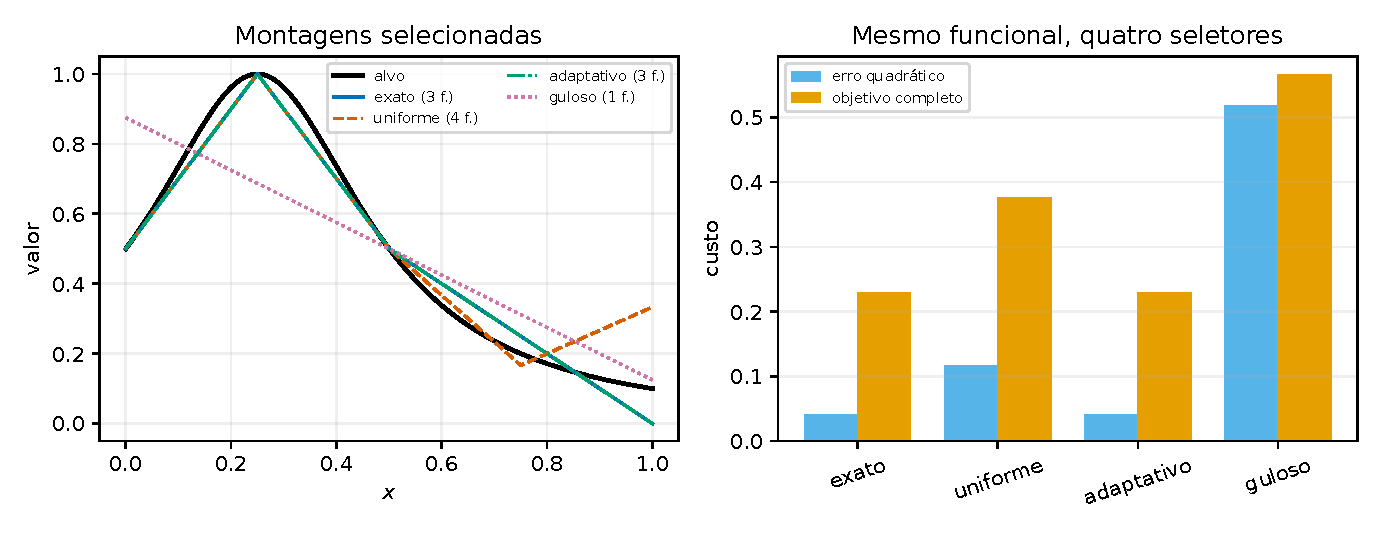
\includegraphics[width=\linewidth]{figuras/artigo_2/fig02_comparacao_seletores.pdf}
 \caption{À esquerda, o alvo e as quatro montagens. À direita, erro quadrático e objetivo completo. As decisões usam racionais exatos; o desenho usa ponto flutuante.}
 \label{artigo_2:fig:selector-comparison}
\end{figure}

As montagens da regressão aparecem na
\cref{artigo_2:fig:selector-comparison}; os valores exatos correspondentes estão na
\cref{artigo_2:tab:selector-comparison}.

\subsection{Propriedades verificadas}

A regressão confirma o mínimo do catálogo e o reaproveitamento de subproblemas. Na instância examinada, o candidato guloso permanece na raiz, enquanto duas subdivisões coordenadas reduzem o custo.

\subsection{Robustez sob truncagem do catálogo}
\label{artigo_2:sec:robustness}

Na instância $(D,H)=(3,4)$, a geometria do catálogo admite $11$ árvores e
elimina a malha uniforme mais fina. Para isolar esse efeito, tome
$(D,H)=(2,4)$, que satisfaz as duas
condições da \cref{artigo_2:prop:translation-obstruction} --- $k_0+D+1\le H$ e
$2^D(m_0+1)\le H$ ---, de modo que a árvore completa é integralmente
admissível: nenhuma célula é vazia e as cinco formas de profundidade no máximo
$2$ são viáveis. Com o mesmo alvo e as mesmas penalidades, as quatro rotas
produzem
\[
 0{,}229497,\quad 0{,}376159,\quad 0{,}229497,\quad 0{,}565803,
\]
com $3$, $4$, $3$ e $1$ folhas: exatamente os valores da
\cref{artigo_2:tab:selector-comparison}. O ótimo exato coincide, inclusive no fluxo
binário, com o da instância truncada --- pois suas três
folhas $[0,\tfrac14]$, $[\tfrac14,\tfrac12]$, $[\tfrac12,1]$ nunca descem
abaixo da profundidade $2$.

A truncagem por translação exclui corretamente a malha uniforme de
profundidade $3$, enquanto preserva o ótimo e seu fluxo binário. Em ambas as
instâncias, a rota gulosa implementada permanece presa na raiz; os valores indicados são os dessas duas instâncias.

\section{Erro interpolatório ótimo em árvores estritamente diádicas}
\label{artigo_2:sec:dyadic-asymptotic}

Fixe primeiro o objeto cuja constante será determinada. Para uma célula
diádica $J=[a,b]$ e $f\in C(J)$, denote por $P_Jf$ a reta que interpola
$f(a)$ e $f(b)$ e ponha
\begin{equation}
 e_f(J)=\|f-P_Jf\|_{\infty,J}.
 \label{artigo_2:eq:local-interpolation-error}
\end{equation}
Se $\Lambda$ é o conjunto de folhas de uma árvore diádica finita com raiz
$K$, as retas $P_Jf$, $J\in\Lambda$, concordam nos nós compartilhados e
definem o interpolante contínuo $P_\Lambda f$. Defina
\begin{equation}
 E_N^{\rm dia}(f)_\infty
 =\min_{\substack{\Lambda\text{ árvore diádica}\\ |\Lambda|\le N}}
   \|f-P_\Lambda f\|_{\infty,K}
 =\min_{\substack{\Lambda\text{ árvore diádica}\\ |\Lambda|\le N}}
   \max_{J\in\Lambda}e_f(J).
 \label{artigo_2:eq:optimal-dyadic-interpolation}
\end{equation}
O mínimo existe: há apenas um número finito de árvores binárias ordenadas e
cheias com no máximo $N$ folhas, e uma árvore com $n$ folhas tem profundidade
no máximo $n-1$.

O sobrescrito ``dia'' distingue \eqref{artigo_2:eq:optimal-dyadic-interpolation} do
erro truncado \eqref{artigo_2:eq:truncated-tree-error}. O primeiro otimiza a
\emph{árvore} e fixa em cada folha a reta interpoladora real; o segundo
otimiza simultaneamente árvore e rótulos racionais de altura no máximo $H$.
As constantes abaixo pertencem ao primeiro problema.
Elas serão comparadas com a referência de nós livres apresentada nas preliminares; a questão aqui é precisamente o custo adicional de
restringir todos os nós a uma árvore diádica.

\subsection{A árvore de limiar é exatamente mínima}

Para $\varepsilon>0$, construa $T_\varepsilon(f)$ recursivamente: uma célula
$J$ é mantida como folha quando $e_f(J)\le\varepsilon$ e é substituída por
seus dois filhos quando $e_f(J)>\varepsilon$. Denote por
\begin{equation}
 n_f(\varepsilon)=|\Lambda(T_\varepsilon(f))|
 \label{artigo_2:eq:threshold-count}
\end{equation}
o número de folhas. Essa regra usa o erro local \emph{exato}; o refinamento
certificado da descrição do refinamento certificado em \citet{artigo_2-oliveiraI} usa o majorante $|J|^2M(J)/8$.

% MAPA artigo_2:11.1
\begin{theorem}[minimalidade exata do limiar]\label{map:artigo_2:11.1}
\label{artigo_2:thm:threshold-optimality}
Se $f\in C(K)$, então $T_\varepsilon(f)$ é finita e é a única árvore
menos refinada (\emph{coarsest}) cuja interpolação tem erro no máximo $\varepsilon$. Em particular,
ela possui o menor número de folhas entre todas as árvores viáveis e
\begin{equation}
 E_N^{\rm dia}(f)_\infty\le\varepsilon
 \quad\Longleftrightarrow\quad
 n_f(\varepsilon)\le N,
 \qquad
 E_N^{\rm dia}(f)_\infty
 =\inf\{\varepsilon>0:n_f(\varepsilon)\le N\}.
 \label{artigo_2:eq:threshold-inversion}
\end{equation}
\end{theorem}

\begin{proof}
Se $\omega_f$ é o módulo de continuidade de $f$, a combinação convexa que
define $P_Jf$ dá
\[
 e_f(J)\le\omega_f(|J|).
\]
Logo todas as células de profundidade suficientemente grande satisfazem o
limiar, e a recursão termina. Quando $f\in C^2$, vale ainda a cota mais
precisa
\begin{equation}
 e_f(J)\le \frac{|J|^2}{8}\|f''\|_{\infty,J}.
 \label{artigo_2:eq:local-upper-basic}
\end{equation}

Se $e_f(J)>\varepsilon$, nenhuma árvore viável pode manter $J$ como folha;
ela é obrigada a subdividi-la. Se $e_f(J)\le\varepsilon$, manter $J$ já é
viável e usa menos folhas que qualquer subdivisão própria. Aplicar essa
dicotomia recursivamente prova, por indução na subárvore finita produzida,
que toda árvore viável refina $T_\varepsilon(f)$. Isso dá unicidade da árvore menos
refinada e minimalidade do número de folhas. A equivalência e a inversão seguem da
definição de \eqref{artigo_2:eq:optimal-dyadic-interpolation}.
\end{proof}

O \cref{artigo_2:thm:threshold-optimality} aplica-se ao funcional uniforme local: a
poda por limiar é exata porque a
viabilidade em norma uniforme é a conjunção dos testes locais
$e_f(J)\le\varepsilon$, e toda falha obriga a mesma subdivisão. Esse problema
escalar é uma especialização da recorrência min--max de
\cref{artigo_2:sec:variable-dp} na qual os
rótulos das folhas já foram fixados pelos dados interpolados. A literatura de
aproximação em árvores enfatiza que, para objetivos mais gerais, árvores
ótimas e algoritmos adaptativos quase ótimos são noções distintas
\citep{artigo_1-cohen2001,artigo_1-binev2004}.

\subsection{Lema local e funcional de curvatura}

Escreva
\[
 \omega_{f''}(t)=\sup_{|x-y|\le t}|f''(x)-f''(y)|,
 \qquad
 I(f)=\int_K\sqrt{|f''(x)|}\,\dd x.
\]

% MAPA artigo_2:11.2
\begin{lemma}[expansão local uniforme]\label{map:artigo_2:11.2}
\label{artigo_2:lem:local-asymptotic-error}
Para toda célula $J\subseteq K$ e todo $x\in J$,
\begin{equation}
 \left|e_f(J)-\frac{|f''(x)|}{8}|J|^2\right|
 \le \frac{\omega_{f''}(|J|)}{8}|J|^2.
 \label{artigo_2:eq:local-asymptotic-error}
\end{equation}
\end{lemma}

\begin{proof}
Seja $q_x$ o polinômio quadrático com $q_x''\equiv f''(x)$ obtido do jato de
$f$ em $x$. Como a interpolação reproduz funções afins,
\[
 \|q_x-P_Jq_x\|_{\infty,J}=\frac{|f''(x)|}{8}|J|^2.
\]
Aplicar \eqref{artigo_2:eq:local-upper-basic} a $f-q_x$ dá
\[
 \|(f-P_Jf)-(q_x-P_Jq_x)\|_{\infty,J}
 \le\frac{|J|^2}{8}\|f''-f''(x)\|_{\infty,J}.
\]
A desigualdade triangular inversa para normas conclui.
\end{proof}

\subsection{O envelope assintótico geral}

% MAPA artigo_2:11.3
\begin{theorem}[envelope diádico universal e agudo]\label{map:artigo_2:11.3}
\label{artigo_2:thm:general-dyadic-envelope}
Se $f\in C^2(K)$ e $I(f)>0$, então
\begin{align}
 \frac{I(f)}{\sqrt8}
 &\le \liminf_{\varepsilon\downarrow0}
       \sqrt\varepsilon\,n_f(\varepsilon)
 \le \limsup_{\varepsilon\downarrow0}
       \sqrt\varepsilon\,n_f(\varepsilon)
 \le \frac{I(f)}{\sqrt2},
 \label{artigo_2:eq:threshold-envelope}\\
 \frac{I(f)^2}{8}
 &\le \liminf_{N\to\infty}N^2E_N^{\rm dia}(f)_\infty
 \le \limsup_{N\to\infty}N^2E_N^{\rm dia}(f)_\infty
 \le \frac{I(f)^2}{2}.
 \label{artigo_2:eq:budget-envelope}
\end{align}
As afirmações continuam válidas se $f''$ possui zeros ou muda de sinal. Se
$I(f)=0$, então $f$ é afim e ambos os erros são identicamente zero.
\end{theorem}

\begin{proof}
Fixe uma partição uniforme diádica $\mathcal Q_q$ de $K$ e ponha
\[
 m_Q=\min_Q|f''|,
 \qquad M_Q=\max_Q|f''|,
 \qquad
 S_q=\sum_{Q\in\mathcal Q_q}|Q|\sqrt{m_Q},
 \quad U_q=\sum_{Q\in\mathcal Q_q}|Q|\sqrt{M_Q}.
\]
Por continuidade de $\sqrt{|f''|}$, $S_q\to I(f)$ e $U_q\to I(f)$.

Considere primeiro $Q$ com $m_Q>0$. O sinal de $f''$ é constante em $Q$.
Para $\varepsilon$ suficientemente pequeno, todos os ancestrais diádicos
próprios de $Q$ têm erro maior que $\varepsilon$: cada um contém um trecho
de curvatura não nula e, portanto, $f$ não é afim nele. Assim, as folhas de
$T_\varepsilon(f)$ que cobrem $Q$ estão contidas em $Q$. No ponto médio de
uma dessas folhas $J$, a fórmula do erro de interpolação fornece
\[
 e_f(J)\ge \frac{m_Q}{8}|J|^2.
\]
Como $e_f(J)\le\varepsilon$, são necessárias pelo menos
$|Q|\sqrt{m_Q}/\sqrt{8\varepsilon}$ folhas para cobrir $Q$. Somando os
$Q$ com $m_Q>0$,
\[
 \liminf_{\varepsilon\downarrow0}
 \sqrt\varepsilon\,n_f(\varepsilon)\ge S_q/\sqrt8.
\]
Fazer $q\to\infty$ dá a primeira desigualdade de
\eqref{artigo_2:eq:threshold-envelope}. Esse argumento também explica por que zeros e
mudanças de sinal não precisam ser excluídos: as células com $m_Q=0$ são
omitidas na soma inferior, e sua contribuição reaparece no limite de Riemann.

Para a cota superior, refine cada $Q\in\mathcal Q_q$ uniformemente até o
primeiro nível $r_Q$ para o qual
\[
 \frac{M_Q|Q|^2}{8}\,4^{-r_Q}\le\varepsilon.
\]
Essa é uma árvore viável por \eqref{artigo_2:eq:local-upper-basic}. Quando
$M_Q|Q|^2/8>\varepsilon$,
\[
 2^{r_Q}<2\sqrt{\frac{M_Q|Q|^2}{8\varepsilon}}
 =\frac{|Q|\sqrt{M_Q}}{\sqrt{2\varepsilon}};
\]
quando a desigualdade falha, usa-se uma única folha. Pela minimalidade do
\cref{artigo_2:thm:threshold-optimality},
\[
 n_f(\varepsilon)
 \le 2^q+\frac{U_q}{\sqrt{2\varepsilon}}.
\]
Primeiro faça $\varepsilon\downarrow0$ e depois $q\to\infty$ para concluir
\eqref{artigo_2:eq:threshold-envelope}.

As partições uniformes e \eqref{artigo_2:eq:local-upper-basic} mostram primeiro que
$E_N^{\rm dia}(f)_\infty\to0$. Se
$\varepsilon_N=E_N^{\rm dia}(f)_\infty$, então
$n_f(\varepsilon_N)\le N$ por \eqref{artigo_2:eq:threshold-inversion}; a cota inferior
acabada de provar dá
$\liminf N^2\varepsilon_N\ge I(f)^2/8$. Para a direção oposta, fixe
$\delta>0$, escolha $q$ com $U_q<I(f)+\delta$ e tome
\[
 \varepsilon=\frac{(I(f)+2\delta)^2}{2N^2}.
\]
Para $N$ grande, a estimativa anterior fornece
$n_f(\varepsilon)\le N$. Logo $E_N^{\rm dia}\le\varepsilon$ pela inversão.
Fazer $N\to\infty$ e depois $\delta\downarrow0$ prova a última desigualdade
de \eqref{artigo_2:eq:budget-envelope}.
\end{proof}

Uma função quadrática realiza os dois extremos de \eqref{artigo_2:eq:budget-envelope} e todos os valores intermediários, como mostra a seção seguinte.

\section{Casos exatos, fases diádicas e validação}
\label{artigo_2:sec:dyadic-exact-cases}

\subsection{Curvatura constante: resposta completa}

% MAPA artigo_2:12.1
\begin{theorem}[lei exata e intervalo de acumulação]\label{map:artigo_2:12.1}
\label{artigo_2:thm:quadratic-dyadic-constant}
Se $K$ é uma célula diádica de comprimento $L$ e
$q''\equiv\kappa\ne0$ em $K$, ponha
\begin{equation}
 A=\frac{|\kappa|L^2}{8}.
 \label{artigo_2:eq:quadratic-A}
\end{equation}
Então, para todo $N\ge1$,
\begin{equation}
 E_N^{\rm dia}(q)_\infty
 =A\,4^{-\lfloor\log_2N\rfloor}.
 \label{artigo_2:eq:quadratic-exact-law}
\end{equation}
Consequentemente,
\begin{equation}
 \liminf_{N\to\infty}N^2E_N^{\rm dia}(q)_\infty=A,
 \qquad
 \limsup_{N\to\infty}N^2E_N^{\rm dia}(q)_\infty=4A,
 \label{artigo_2:eq:quadratic-liminf-limsup}
\end{equation}
e o conjunto completo dos valores de acumulação de
$N^2E_N^{\rm dia}(q)_\infty$ é o intervalo $[A,4A]$. Em particular, a
constante obtida por um limite simples não existe.
\end{theorem}

\begin{proof}
Em uma folha $J$ de comprimento $\ell$,
\begin{equation}
 e_q(J)=\frac{|\kappa|}{8}\ell^2.
 \label{artigo_2:eq:quadratic-local-exact}
\end{equation}
Se $r=\lfloor\log_2N\rfloor$, a árvore uniforme de profundidade $r$ usa
$2^r\le N$ folhas, todas de comprimento $L2^{-r}$, e atinge o lado direito
de \eqref{artigo_2:eq:quadratic-exact-law}. Para obter erro estritamente menor seria
necessário que toda célula da profundidade $r$ fosse subdividida, pois
qualquer uma mantida como folha ainda teria o erro de
\eqref{artigo_2:eq:quadratic-exact-law}. Isso exigiria $2^{r+1}>N$ folhas. A fórmula
está provada.

Agora
\[
 N^2E_N^{\rm dia}=A\left(\frac{N}{2^r}\right)^2,
 \qquad 2^r\le N<2^{r+1}.
\]
As escolhas $N=2^r$ e $N=2^{r+1}-1$ dão os extremos de
\eqref{artigo_2:eq:quadratic-liminf-limsup}. Para qualquer $t\in[1,2)$, tomar
$N_r=\lfloor t2^r\rfloor$ produz o limite $At^2$; o valor $4A$ é obtido
pela segunda sequência. Isso dá exatamente $[A,4A]$.
\end{proof}

Como $I(q)=L\sqrt{|\kappa|}$, os extremos são
$A=I(q)^2/8$ e $4A=I(q)^2/2$. Logo ambas as constantes do
\cref{artigo_2:thm:general-dyadic-envelope} são agudas. Em contraste, a referência de
nós livres tem a constante inferior $I(q)^2/8$: a restrição diádica a
recupera nas potências de dois, mas perde um fator que tende a quatro logo
antes da potência seguinte.

A formulação dual em tolerância também é exata:
\begin{equation}
 n_q(\varepsilon)
 =2^{\max\{0,\lceil\log_4(A/\varepsilon)\rceil\}}.
 \label{artigo_2:eq:quadratic-threshold-count}
\end{equation}
Ela fornece a contagem exata do ótimo interpolatório e coincide, em curvatura
constante, com a lei de refinamento certificado da descrição do refinamento certificado em \citet{artigo_2-oliveiraI}.

\begin{table}[t]
 \centering
 \caption{Lei exata para $q(x)=x^2$ em $[0,1]$, quando $A=1/4$.}
 \label{artigo_2:tab:quadratic-exact}
 \small
 \begin{tabular}{rrrr}
\toprule
$N$ & $\lfloor\log_2N\rfloor$ & $E_N^{\rm dia}(q)_\infty$ & $N^2E_N/A$ \\
\midrule
1 & 0 & $\frac{1}{4}$ & 1{,}000000 \\
2 & 1 & $\frac{1}{16}$ & 1{,}000000 \\
3 & 1 & $\frac{1}{16}$ & 2{,}250000 \\
4 & 2 & $\frac{1}{64}$ & 1{,}000000 \\
7 & 2 & $\frac{1}{64}$ & 3{,}062500 \\
8 & 3 & $\frac{1}{256}$ & 1{,}000000 \\
15 & 3 & $\frac{1}{256}$ & 3{,}515625 \\
16 & 4 & $\frac{1}{1024}$ & 1{,}000000 \\
31 & 4 & $\frac{1}{1024}$ & 3{,}753906 \\
\bottomrule
\end{tabular}

\end{table}

\begin{figure}[t]
 \centering
 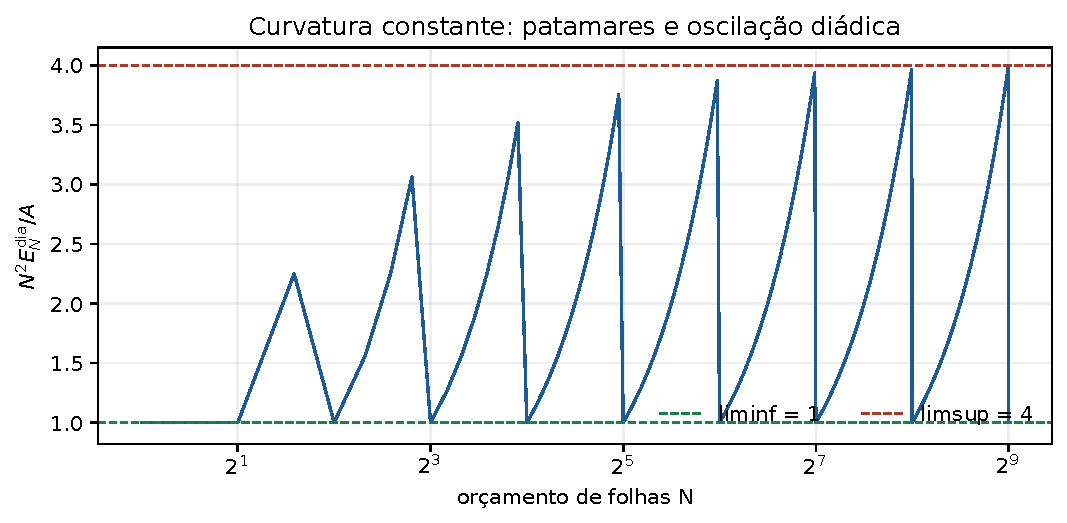
\includegraphics[width=.88\linewidth]{figuras/artigo_2/fig03_constante_quadratica.pdf}
 \caption{A normalização $N^2E_N^{\rm dia}/A$ reinicia em $1$ nas potências
 de dois e se aproxima de $4$ antes da potência seguinte.}
 \label{artigo_2:fig:quadratic-sawtooth}
\end{figure}

A \cref{artigo_2:tab:quadratic-exact} lista os valores racionais da lei, e a
\cref{artigo_2:fig:quadratic-sawtooth} exibe a oscilação normalizada entre as fases
diádicas consecutivas.

\subsection{Quadráticas por partes e lei de fase}

O caso seguinte separa a oscilação causada por uma única escala daquela
produzida por regiões com curvaturas diferentes.

% MAPA artigo_2:12.2
\begin{theorem}[contagem exata em uma malha diádica base]\label{map:artigo_2:12.2}
\label{artigo_2:thm:piecewise-quadratic-count}
Seja $\mathcal Q_{q_0}$ a partição uniforme de $K=[0,1]$ em células
$Q_i$ de comprimento $2^{-q_0}$. Suponha que $f\in C^1(K)$ seja quadrática
em cada $Q_i$ e
\[
 f''|_{\mathring Q_i}=\kappa_i\ne0,
 \qquad
 A_i=\frac{|\kappa_i||Q_i|^2}{8}.
\]
Existe $\varepsilon_0>0$ tal que, para
$0<\varepsilon<\varepsilon_0$,
\begin{equation}
 n_f(\varepsilon)
 =\sum_i2^{\lceil\log_4(A_i/\varepsilon)\rceil}.
 \label{artigo_2:eq:piecewise-count-law}
\end{equation}
Se $s=-\log_4\varepsilon$ e $a_i=\log_4A_i$, então
\begin{equation}
 \sqrt\varepsilon\,n_f(\varepsilon)
 =\Phi(s),
 \qquad
 \Phi(s)=\sum_i\sqrt{A_i}\,
 2^{\lceil s+a_i\rceil-(s+a_i)}.
 \label{artigo_2:eq:piecewise-phase-law}
\end{equation}
A função $\Phi$ é $1$-periódica e não constante. Portanto nem mesmo a
normalização em tolerância possui, em geral, um limite simples.
\end{theorem}

\begin{proof}
Todo ancestral da malha base que contém algum $Q_i$ é não afim, logo possui
erro local positivo. Como há apenas um número finito desses ancestrais,
escolha $\varepsilon_0$ menor que todos os seus erros e que todos os $A_i$.
O \cref{artigo_2:thm:threshold-optimality} obriga então a árvore de limiar a alcançar
cada $Q_i$. Dentro de $Q_i$, a identidade
\eqref{artigo_2:eq:quadratic-local-exact} mostra que são necessárias e suficientes
$2^{\lceil\log_4(A_i/\varepsilon)\rceil}$ folhas. Somar prova
\eqref{artigo_2:eq:piecewise-count-law}; a reescrita algébrica dá
\eqref{artigo_2:eq:piecewise-phase-law}. A periodicidade segue de
$\lceil s+1+a_i\rceil-(s+1+a_i)=\lceil s+a_i\rceil-(s+a_i)$.
Em qualquer intervalo aberto sem uma das finitíssimas fases de salto, todos
os tetos permanecem fixos e $\Phi$ é um múltiplo positivo de $2^{-s}$;
portanto é estritamente decrescente ali e não pode ser constante.
\end{proof}

% MAPA artigo_2:12.3
\begin{corollary}[fases sincronizadas]\label{map:artigo_2:12.3}
\label{artigo_2:cor:synchronized-phases}
Nas hipóteses do \cref{artigo_2:thm:piecewise-quadratic-count}, suponha ainda que
$A_i/A_j\in4^{\mathbb Z}$ para todos $i,j$. Então
\begin{equation}
 \liminf_{N\to\infty}N^2E_N^{\rm dia}(f)_\infty=\frac{I(f)^2}{8},
 \qquad
 \limsup_{N\to\infty}N^2E_N^{\rm dia}(f)_\infty=\frac{I(f)^2}{2}.
 \label{artigo_2:eq:synchronized-extremes}
\end{equation}
\end{corollary}

\begin{proof}
Seja $A_\ast=\min_iA_i>0$. Pela hipótese de sincronia, $A_i=A_\ast4^{\rho_i}$ com
$\rho_i\in\mathbb Z$, e a minimalidade de $A_\ast$ dá $\rho_i\ge0$. Ponha
$M=\sum_i2^{\rho_i}\ge1$.

Pelo \cref{artigo_2:thm:piecewise-quadratic-count}, existe $\varepsilon_0>0$ tal que,
para $0<\varepsilon<\varepsilon_1:=\min\{\varepsilon_0,A_\ast\}$,
$n_f(\varepsilon)=\sum_i2^{\lceil\log_4(A_i/\varepsilon)\rceil}$. Com
$D(\varepsilon)=\lceil\log_4(A_\ast/\varepsilon)\rceil$ e $\varepsilon<A_\ast$, vale
$\lceil\log_4(A_\ast4^{\rho_i}/\varepsilon)\rceil=\rho_i+D(\varepsilon)$, logo
\[
 n_f(\varepsilon)=M\,2^{D(\varepsilon)},
 \qquad
 D(\varepsilon)\le j\iff A_\ast4^{-j}\le\varepsilon .
\]

Fixe $R_0$ com $A_\ast4^{-R_0}<\varepsilon_1$ e, para $N\ge M2^{R_0}$, ponha
$j(N)=\lfloor\log_2(N/M)\rfloor\ge R_0$. Para $0<\varepsilon<\varepsilon_1$, o
\cref{artigo_2:thm:threshold-optimality} dá
$E_N^{\rm dia}(f)_\infty\le\varepsilon\iff n_f(\varepsilon)\le N\iff
M2^{D(\varepsilon)}\le N\iff D(\varepsilon)\le j(N)\iff A_\ast4^{-j(N)}\le\varepsilon$.
Como $A_\ast4^{-j(N)}<\varepsilon_1$, as duas quantidades têm os mesmos majorantes
em $(0,\varepsilon_1)$, e portanto
\[
 E_N^{\rm dia}(f)_\infty=A_\ast4^{-\lfloor\log_2(N/M)\rfloor}
 \qquad(N\ge M2^{R_0}).
\]
É a lei exata do \cref{artigo_2:thm:quadratic-dyadic-constant}, com $A$ substituído
por $A_\ast$ e o orçamento medido em unidades de $M$. Se
$M2^j\le N<M2^{j+1}$, então $M^2A_\ast\le N^2E_N^{\rm dia}(f)_\infty<4M^2A_\ast$;
o valor $M^2A_\ast$ é atingido em $N=M2^j$ e
$(M2^{j+1}-1)^2A_\ast4^{-j}\to4M^2A_\ast$. Logo
\[
 \liminf_{N\to\infty}N^2E_N^{\rm dia}(f)_\infty=M^2A_\ast,
 \qquad
 \limsup_{N\to\infty}N^2E_N^{\rm dia}(f)_\infty=4M^2A_\ast .
\]
Finalmente, no interior de cada $Q_i$ tem-se $|f''|=|\kappa_i|$, de modo que
\[
 I(f)=\sum_i\sqrt{|\kappa_i|}\,|Q_i|=\sum_i\sqrt{8A_i}
 =\sqrt{8A_\ast}\sum_i2^{\rho_i}=\sqrt{8A_\ast}\,M,
\]
isto é, $M^2A_\ast=I(f)^2/8$ e $4M^2A_\ast=I(f)^2/2$, o que prova
\eqref{artigo_2:eq:synchronized-extremes}. A demonstração usa apenas a contagem
exata do \cref{artigo_2:thm:piecewise-quadratic-count} e a periodicidade em
$4^{\mathbb Z}$; não recorre ao envelope do
\cref{artigo_2:thm:general-dyadic-envelope}, cuja hipótese $C^2$ uma quadrática por
partes pode não satisfazer.
\end{proof}

A presença de sinais diferentes entre os $\kappa_i$ não altera essas
fórmulas: os erros locais dependem de $|\kappa_i|$. Para uma função global
$C^2$, uma mudança de sinal passa por zeros e a lei finita por fases deixa de
ser literalmente aplicável, mas o \cref{artigo_2:thm:general-dyadic-envelope} continua
válido sem alteração.

\begin{figure}[t]
 \centering
 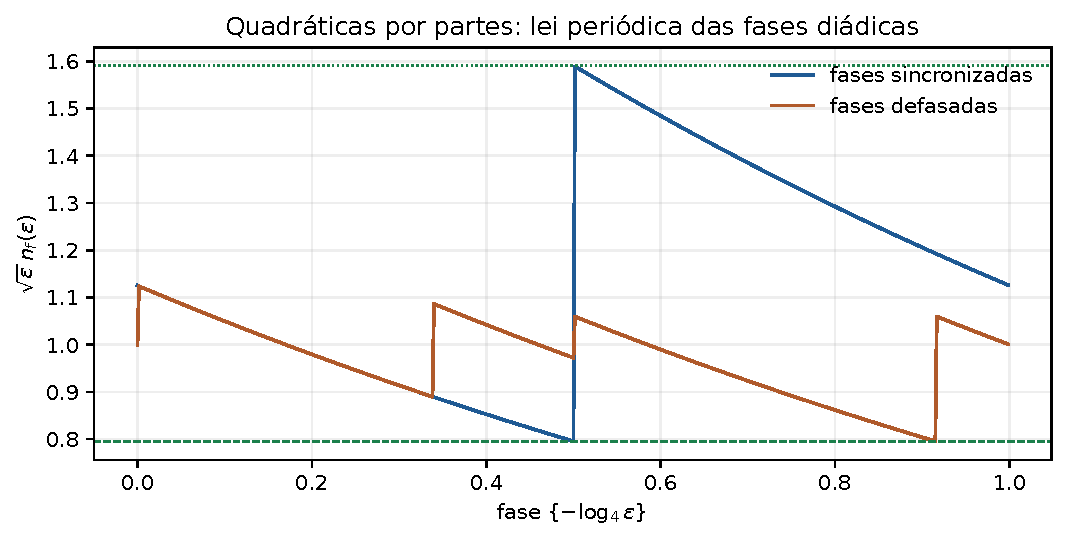
\includegraphics[width=.88\linewidth]{figuras/artigo_2/fig04_fases_piecewise.pdf}
 \caption{A lei \eqref{artigo_2:eq:piecewise-phase-law} em uma família sincronizada e
 outra defasada. Deslocar $-\log_4\varepsilon$ por uma unidade repete
 exatamente o perfil.}
 \label{artigo_2:fig:piecewise-phases}
\end{figure}

A sincronização e a defasagem previstas por
\eqref{artigo_2:eq:piecewise-phase-law} são comparadas na
\cref{artigo_2:fig:piecewise-phases}.

\subsection{Implementação e auditorias independentes}

O programa \path{verificacao/constante_diadica.py} implementa duas rotas que não
reutilizam a mesma recorrência: a árvore menos refinada do
\cref{artigo_2:thm:threshold-optimality} e uma programação dinâmica por número exato
de folhas,
\begin{equation}
 D(J,1)=e_f(J),\qquad
 D(J,n)=\min_{n_L+n_R=n}\max\{D(J_L,n_L),D(J_R,n_R)\}.
 \label{artigo_2:eq:independent-tree-dp}
\end{equation}
Para funções quadráticas por partes, $f$, $f'$, todos os pontos críticos e
todos os erros locais são calculados com \texttt{Fraction}. A fórmula
quadrática foi comparada com \eqref{artigo_2:eq:independent-tree-dp} para
$1\le N\le14$; a lei por partes foi confrontada com a construção explícita
do limiar em 14 escalas e a inversão do limiar foi comparada com a DP para
$1\le N\le12$.

Os dois diagnósticos $C^2$ usam apenas ponto flutuante determinístico para
avaliar extremos analíticos: $e^x$, cuja curvatura é estritamente positiva,
e $(x-1/2)^3$, cuja segunda derivada muda de sinal. Eles não participam de
nenhuma prova de igualdade; verificam apenas que os valores finitos
$\varepsilon n_f(\varepsilon)^2$ permanecem dentro do envelope teórico nas
$400$ tolerâncias examinadas.

% MAPA artigo_2:12.4
\begin{remark}[agudeza uniforme e comportamento pontual]\label{map:artigo_2:12.4}
\label{artigo_2:rem:envelope-not-pointwise}
O \cref{artigo_2:thm:general-dyadic-envelope} é agudo \emph{uniformemente sobre a
classe} $C^2$: a mesma função quadrática do
\cref{artigo_2:thm:quadratic-dyadic-constant} realiza $I(f)^2/8$ e $I(f)^2/2$ ao longo
de subsequências. Logo as duas constantes são ótimas em teoremas uniformes
sobre $C^2$. Para uma função fixa, o conjunto de acumulação pode ser um
subconjunto próprio do envelope.

No modelo finito do \cref{artigo_2:thm:piecewise-quadratic-count}, essa distinção pode
ser tornada exata. Ponha $w_i=\sqrt{A_i}$ e considere os resíduos de
$a_i=\log_4A_i$ módulo $1$. Cada fator
\[
 g(s+a_i)=2^{\lceil s+a_i\rceil-(s+a_i)}
\]
pertence a $[1,2)$ e vale $1$ precisamente quando $s+a_i\in\mathbb Z$. Se os
resíduos não são todos iguais, não existe fase que torne simultaneamente
todos os fatores iguais a $1$, nem uma sequência de fases que os faça tender
simultaneamente a $2$. Como há apenas um número finito de fases de salto no
círculo, existem $\delta_-,\delta_+>0$ tais que
\[
 \frac{I(f)}{\sqrt8}+\delta_-
 \le \Phi(s)
 \le \frac{I(f)}{\sqrt2}-\delta_+
 \qquad(s\in\mathbb R).
\]
Assim, a normalização dual $\varepsilon n_f(\varepsilon)^2$ permanece
estritamente dentro do envelope para todas as tolerâncias suficientemente
pequenas nessa família defasada. No caso sincronizado, a condição
$A_i/A_j\in4^{\mathbb Z}$ do \cref{artigo_2:cor:synchronized-phases} alinha os
resíduos e permite recuperar os extremos.

A prova finita usa o número discreto de fases de salto e, portanto, é
específica da curvatura quadrática por partes. A
\cref{artigo_2:tab:smooth-diagnostics} registra que, em $400$ tolerâncias entre
$10^{-3}$ e $10^{-10}$, os dois exemplos suaves permanecem estritamente no
interior. A caracterização, para $f$ dada, do conjunto exato de acumulação de
$N^2E_N^{\rm dia}(f)_\infty$ dentro de
$[I(f)^2/8,\allowbreak I(f)^2/2]$ constitui o problema de fases para curvatura variável.
\end{remark}

\begin{table}[t]
 \centering
 \caption{Diagnósticos determinísticos em 400 tolerâncias entre
 $10^{-3}$ e $10^{-10}$. As colunas externas são teóricas.}
 \label{artigo_2:tab:smooth-diagnostics}
 \small
 \begin{tabular}{lrrr}
\toprule
função & $I(f)^2/8$ & faixa observada de $\varepsilon n_f(\varepsilon)^2$ & $I(f)^2/2$ \\
\midrule
$e^x$ & 0{,}210420 & [0{,}339008; 0{,}515293] & 0{,}841679 \\
$(x-\frac{1}{2})^3$ & 0{,}166667 & [0{,}275877; 0{,}417099] & 0{,}666667 \\
\bottomrule
\end{tabular}

\end{table}

\begin{figure}[t]
 \centering
 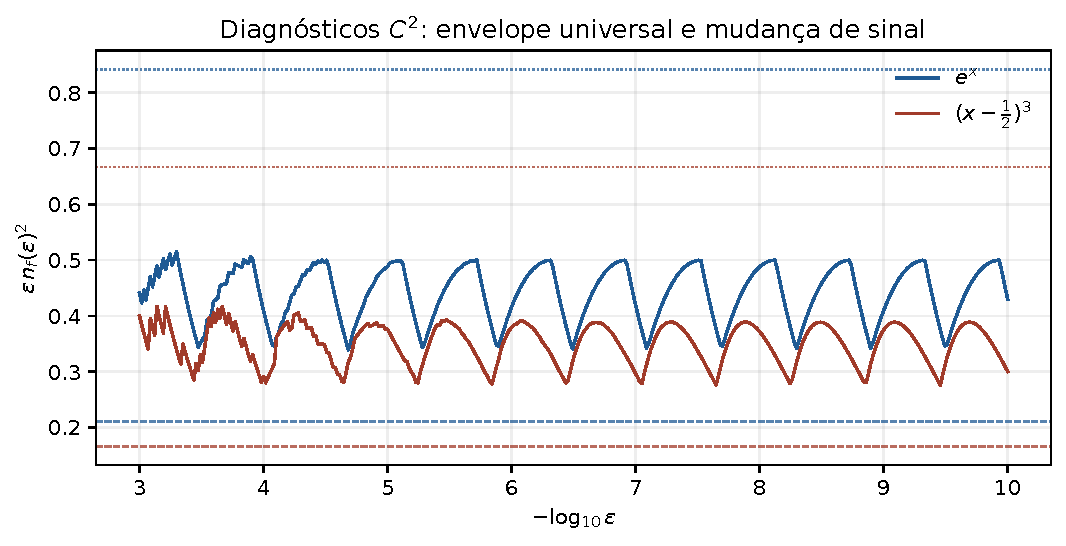
\includegraphics[width=.88\linewidth]{figuras/artigo_2/fig05_envelope_c2.pdf}
 \caption{Diagnósticos para curvatura positiva e para mudança de sinal. As
 linhas tracejadas e pontilhadas são, respectivamente, $I(f)^2/8$ e
 $I(f)^2/2$.}
 \label{artigo_2:fig:c2-envelope}
\end{figure}

Os dois exemplos suaves da \cref{artigo_2:fig:c2-envelope} permanecem dentro do
envelope teórico em todas as tolerâncias auditadas.

\begin{table}[t]
 \centering
 \caption{Auditoria executável das constantes diádicas.}
 \label{artigo_2:tab:dyadic-constants-audit}
 \small
 \begin{tabularx}{\linewidth}{@{}Xr@{}}
\toprule
Verificação & resultado \\
\midrule
Fórmula quadrática $=$ DP independente & true \\
Limiar quadrático $=$ contagem fechada & true \\
Contagem por partes $=$ árvore de limiar & true \\
DP por partes $=$ inversão do limiar & true \\
Fases sincronizadas atingem os dois extremos & true \\
Diagnóstico $C^2$ positivo dentro do envelope & true \\
Mudança de sinal dentro do envelope & true \\
Varreduras suaves estritamente interiores (400 pontos) & true \\
Execução sem números pseudoaleatórios & true \\
\bottomrule
\end{tabularx}

\end{table}

A \cref{artigo_2:tab:dyadic-constants-audit} reúne, em uma única trilha, as
identidades exatas e os testes independentes desta seção.

\subsection{Compatibilidade com a altura aritmética}

Os teoremas desta seção permitem todos os descendentes da raiz. Na biblioteca
$\Library$, uma malha uniforme de profundidade relativa $r$ em
$K=J_{k_0,m_0}$, $m_0\ge0$, só está espacialmente disponível quando
\[
 H\ge k_0+r+1,
 \qquad H\ge2^r(m_0+1)
\]
pela \cref{artigo_2:prop:translation-obstruction}. Como as escalas relevantes têm
$2^r\asymp N$, a segunda condição já força $H=\Omega(N(m_0+1))$, antes de
se contabilizar a altura necessária para racionalizar os valores nodais.
Assim, a passagem de \eqref{artigo_2:eq:budget-envelope} para uma agenda $H(N)$ inclui
esse acoplamento geométrico.

Para cada árvore fixa, o teorema de racionalização da \cref{artigo_2:sec:assemblies}
aproxima os valores nodais reais por racionais compartilhados e aproxima
$P_\Lambda f$ arbitrariamente bem por uma montagem da biblioteca. Os
interpolantes pertencem, portanto, à aderência quando a altura cresce. O
problema interpolatório \eqref{artigo_2:eq:optimal-dyadic-interpolation} e o melhor
erro racional com deslocamentos nodais são objetos distintos; a constante
assintótica do segundo sob uma agenda fixa de altura permanece em aberto.
\section{Verificações de codificação e entropia}
\label{artigo_2:sec:coding-validation}
Os registros desta seção acompanham o programa \path{verificacao/reproduzir_curvas.py}. As verificações usam aritmética racional para os formatos e parâmetros; as curvas e as sondas de distorção são diagnósticos numéricos.

\subsection{Roundtrip dos formatos de codificação}

Os codificadores de \cref{artigo_2:subsec:coding-formats} e seus decodificadores foram
executados em $4096$ montagens racionais de teste. Em
todos os casos, o fluxo atômico recuperou a assinatura linear por partes e os
dois fluxos ReLU recuperaram exatamente cada \texttt{Fraction} da rede. Foram
também verificadas, parâmetro a parâmetro, as cotas
\eqref{artigo_2:eq:slope-jump-height}--\eqref{artigo_2:eq:intercept-height}.

A fatia $N=2$ da família de \eqref{artigo_2:eq:coding-gap-family} permite comparar os
comprimentos sem regressão nem ajuste assintótico. A
\cref{artigo_2:tab:codificacoes-pt} dá os valores exatos e a
\cref{artigo_2:fig:codificacoes-pt} mostra as ordens de crescimento:
\begin{table}[t]
\centering
\caption{Comprimentos exatos dos três fluxos prefix-free na família crítica.}
\label{artigo_2:tab:codificacoes-pt}
\small
\begin{tabular}{rrrrr}
\toprule
$H$ & $L_{\rm atom}$ & $L_{\rm ReLU,str}$ & $L_{\rm ReLU,rat}$ & razão rat./str.\\
\midrule
4 & 29 & 31 & 35 & 1{,}129\\
8 & 33 & 35 & 51 & 1{,}457\\
16 & 37 & 39 & 83 & 2{,}128\\
32 & 41 & 43 & 147 & 3{,}419\\
64 & 45 & 47 & 275 & 5{,}851\\
128 & 49 & 51 & 531 & 10{,}412\\
\bottomrule
\end{tabular}

\end{table}

\begin{figure}[t]
 \centering
 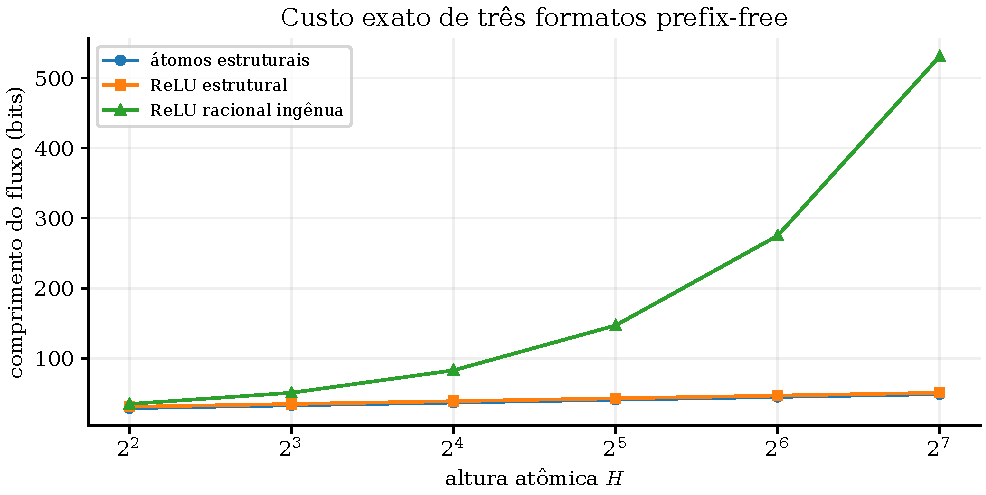
\includegraphics[width=.82\linewidth]{figuras/artigo_2/fig08_codificacoes.pdf}
 \caption{O par diádico estrutural mantém o custo logarítmico; expandir o
 denominador $2^k$ como parte de uma fração racional produz a sobrecarga
 linear prevista pelo \cref{artigo_2:thm:coding-formats}.}
 \label{artigo_2:fig:codificacoes-pt}
\end{figure}


\subsection{Restrição de curvatura e codebook sem fator logarítmico}

A contagem de \eqref{artigo_2:eq:code-length} restringe os vetores admissíveis pelas diferenças segundas, mantendo os mesmos átomos e grades.

O script avalia quatro sondas determinísticas. Cada uma é reescalada pelo fator
\[\min\{R/\|f\|_\infty,\,M/\|f''\|_\infty\}\]
para que pertença a
$\mathcal F_{R,M}$ com $R=1$ e $M=8$: a quadrática que satura as duas
restrições simultaneamente, dois harmônicos e a função de Runge reescalada.
Antes do reescalamento, a sonda de Runge tem $\|f''\|_\infty=200$. Para cada tolerância, verifica-se que
$\varepsilon/2<\delta\le\varepsilon$, que $Mh^2\le4\varepsilon$, que o erro
nodal não excede $\delta/2$, que valores adjacentes são distintos, que cada
peça é um átomo de inclinação racional não nula e que a distorção fica dentro
de $\varepsilon$.

\begin{table}[t]
\centering
\caption{Sucessores admissíveis por nó e comprimento do índice global reescalado.}
\label{artigo_2:tab:codebook-pt}
\small
\begin{tabular}{rrrrrr}
\toprule
$\varepsilon$ & $N$ & sucessores & distorção & $L_\varepsilon^{\mathrm{global}}\sqrt{\varepsilon}$ & antigo $\cdot\sqrt{\varepsilon}$\\
\midrule
$6{,}250\,10^{-2}$ & 8   & 9 & $3{,}90\,10^{-2}$ & $10{,}68$ & $13{,}50$\\
$1{,}562\,10^{-2}$ & 16  & 9 & $9{,}68\,10^{-3}$ & $10{,}34$ & $17{,}00$\\
$3{,}906\,10^{-3}$ & 32  & 9 & $2{,}26\,10^{-3}$ & $10{,}00$ & $20{,}62$\\
$9{,}766\,10^{-4}$ & 64  & 9 & $6{,}98\,10^{-4}$ & $9{,}74$  & $24{,}38$\\
$2{,}441\,10^{-4}$ & 128 & 9 & $1{,}62\,10^{-4}$ & $9{,}56$  & $28{,}22$\\
\bottomrule
\end{tabular}
\end{table}

Na \cref{artigo_2:tab:codebook-pt}, O número de sucessores
admissíveis por nó, dados os dois valores anteriores, é $9$ em todas as
tolerâncias --- abaixo da constante $K=25$ usada na demonstração, que é
portanto conservadora e não ajustada aos dados. As duas últimas colunas são o
diagnóstico do fator logarítmico: o comprimento do índice global da cota por diferenças segundas,
multiplicado por $\sqrt{\varepsilon}$, permanece limitado e até decresce
levemente, enquanto a contagem termo a termo de cada nó cresce
como $\log(1/\varepsilon)$ na mesma normalização. É exatamente a diferença
entre $O(\varepsilon^{-1/2})$ e $O(\varepsilon^{-1/2}\log(1/\varepsilon))$.


\subsection{Contagem de átomos e otimalidade minimax do endereço}

A \cref{artigo_2:tab:enderecos-pt} confronta a contagem exata $|\Library_H|$ com as cotas do
\cref{artigo_2:lem:atom-count} e compara, no pior caso sobre $\Library_H$, o endereço
aritmético $n$ do gerador $\Gamma$ com o endereço $n^\sharp$ da enumeração por
altura da \cref{artigo_2:def:sharp}. A coluna final registra a cota inferior universal,
quanto ao endereçamento sob o calibre fixado, do
\cref{artigo_2:thm:address-lower}. Os expoentes empíricos, obtidos por regressão de
$\log_2(\cdot)$ contra $\log_2H$ nas últimas linhas, aproximam $6$ para
$|\Library_H|$ e $n^\sharp$ e $8$ para $n$, como previsto.

\begin{table}[t]
\centering
\caption{Contagem de átomos por altura e comprimento de endereço no pior caso.}
\label{artigo_2:tab:enderecos-pt}
\small
\begin{tabular}{rrrrr}
\toprule
$H$ & $|\Library_H|$ & $|\Library_H|/(18H^6)$ & $\max n$ ($\Gamma$) & $\max n^\sharp=$ cota inf.\\
\midrule
2 & 252 & 0{,}2188 & 3231 & 251\\
3 & 3150 & 0{,}2401 & 87\,127 & 3149\\
4 & 14\,168 & 0{,}1922 & 519\,638 & 14\,167\\
6 & 142\,692 & 0{,}1699 & 9\,515\,572 & 142\,691\\
8 & 897\,840 & 0{,}1903 & 113\,062\,957 & 897\,839\\
12 & 9\,192\,456 & 0{,}1710 & 2\,233\,224\,112 & 9\,192\,455\\
16 & 50\,315\,232 & 0{,}1666 & 20\,668\,188\,575 & 50\,315\,231\\
24 & 582\,320\,976 & 0{,}1693 & 534\,070\,940\,833 & 582\,320\,975\\
32 & 3\,378\,271\,680 & 0{,}1748 & 5\,622\,328\,883\,731 & 3\,378\,271\,679\\
48 & 36\,947\,682\,720 & 0{,}1678 & 131\,374\,552\,971\,847 & 36\,947\,682\,719\\
64 & 206\,341\,325\,696 & 0{,}1668 & 1\,289\,353\,431\,661\,883 & 206\,341\,325\,695\\
\bottomrule
\end{tabular}

\end{table}

A \cref{artigo_2:fig:enderecos-pt} torna visível a diferença entre os expoentes do
gerador aritmético e da enumeração por cascas, sempre para o calibre
\eqref{artigo_2:eq:atom-height}.

\begin{figure}[t]
 \centering
 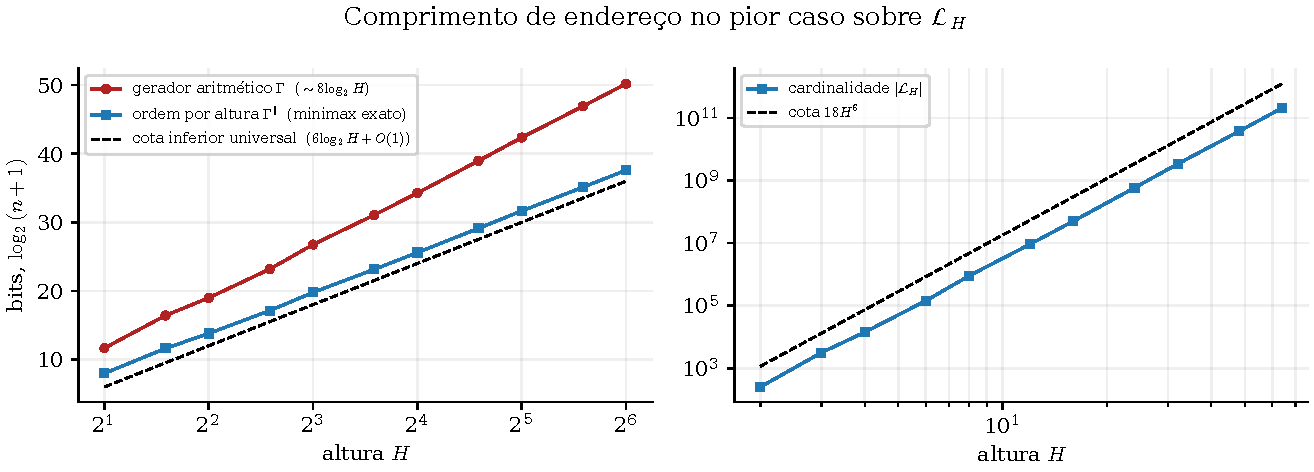
\includegraphics[width=.92\linewidth]{figuras/artigo_2/fig06_enderecos.pdf}
 \caption{Comprimento de endereço no pior caso sobre $\Library_H$. A enumeração
 por altura $\Gamma^\sharp$ acompanha a cota inferior relativa a $\Library_H$ com uma folga
 limitada; o gerador aritmético $\Gamma$ paga um fator constante $4/3$ no
 expoente em troca de inversa em forma fechada.}
 \label{artigo_2:fig:enderecos-pt}
\end{figure}

Foi ainda verificada, para $0\le n^\sharp<20\,000$, a bijetividade de
$\Gamma^\sharp$ nos dois sentidos e a coincidência dos conjuntos
$\Gamma(\{0,\ldots,N\})$ e $\Gamma^\sharp(\{0,\ldots,N'\})$ quando restritos a
uma mesma casca de altura.

\FloatBarrier
\clearpage
\section{Conclusão}
O calibre adotado produz $\Theta(H^6)$ átomos e uma enumeração por altura que minimiza exatamente o pior índice. Os três formatos de codificação explicitam como a representação dos diádicos altera o comprimento da palavra. A restrição de curvatura reduz a cardinalidade do codebook e realiza a ordem entrópica $\varepsilon^{-1/2}$.

Na seleção, os valores racionais de fronteira fornecem estados suficientes para preservar continuidade e admissibilidade. As recorrências calculam o mínimo do catálogo, com desempate canônico e custos separados em operações e bits. A estabilização sob truncagem exige que o mínimo global seja atingido; a seleção exata pode ser descontínua em empates.

Para a interpolação estritamente diádica, o erro normalizado admite o envelope $[I(f)^2/8,\allowbreak I(f)^2/2]$. Curvatura constante e quadráticas por partes explicitam as fases responsáveis pela oscilação. A caracterização das fases para curvatura variável e o efeito de uma agenda fixa sobre o melhor erro racional permanecem questões distintas dos resultados interpolatórios demonstrados.


